\clearpage{\pagestyle{empty}\cleardoublepage}
\chapter{Visualizzazione dei Percorsi Escursionistici}
%%%%%%%%%%%%%%%%%%%%%%%%%%%%%%%%%%%%%%%%%imposta l'intestazione di pagina

% Questo capitolo avrà lo scopo di introdurre l'applicazione web sviluppata, mettendo in evidenza i principali obiettivi, le sfide affrontate e le soluzioni implementate. Inoltre verrà fornita una panoramica delle schermate chiave dell'applicazione.

Questo capitolo avrà lo scopo di introdurre l'applicazione web sviluppata, mettendo in evidenza sia l'ambiente di lavoro (mostrando le varie regole per mantenere un codice pulito e leggibile) sia i principali obiettivi, le sfide affrontate e le soluzioni implementate. Inoltre verrà fornita una panoramica delle schermate chiave dell'applicazione.

\section{Database}

 Lo sviluppo dell'applicazione è iniziata definendo la struttura del database, in quanto base fondamentale di tutto questo progetto.

I dati relativi ai percorsi e ai punti di interesse sono stati forniti dal sito governativo \href{https://geoportale.regione.emilia-romagna.it/catalogo/dati-cartografici/ambiente/percorsi-escursionistici}{”Geo portale Regione Emilia-Romagna”} sotto forma di file \emph{XML}.

La struttura del database finale è illustrata in dettaglio nella figura \ref{fig:database}, e questa rappresentazione visiva fornisce una panoramica chiara e intuitiva della sua organizzazione.

\begin{figure}[h]
\begin{center}                      
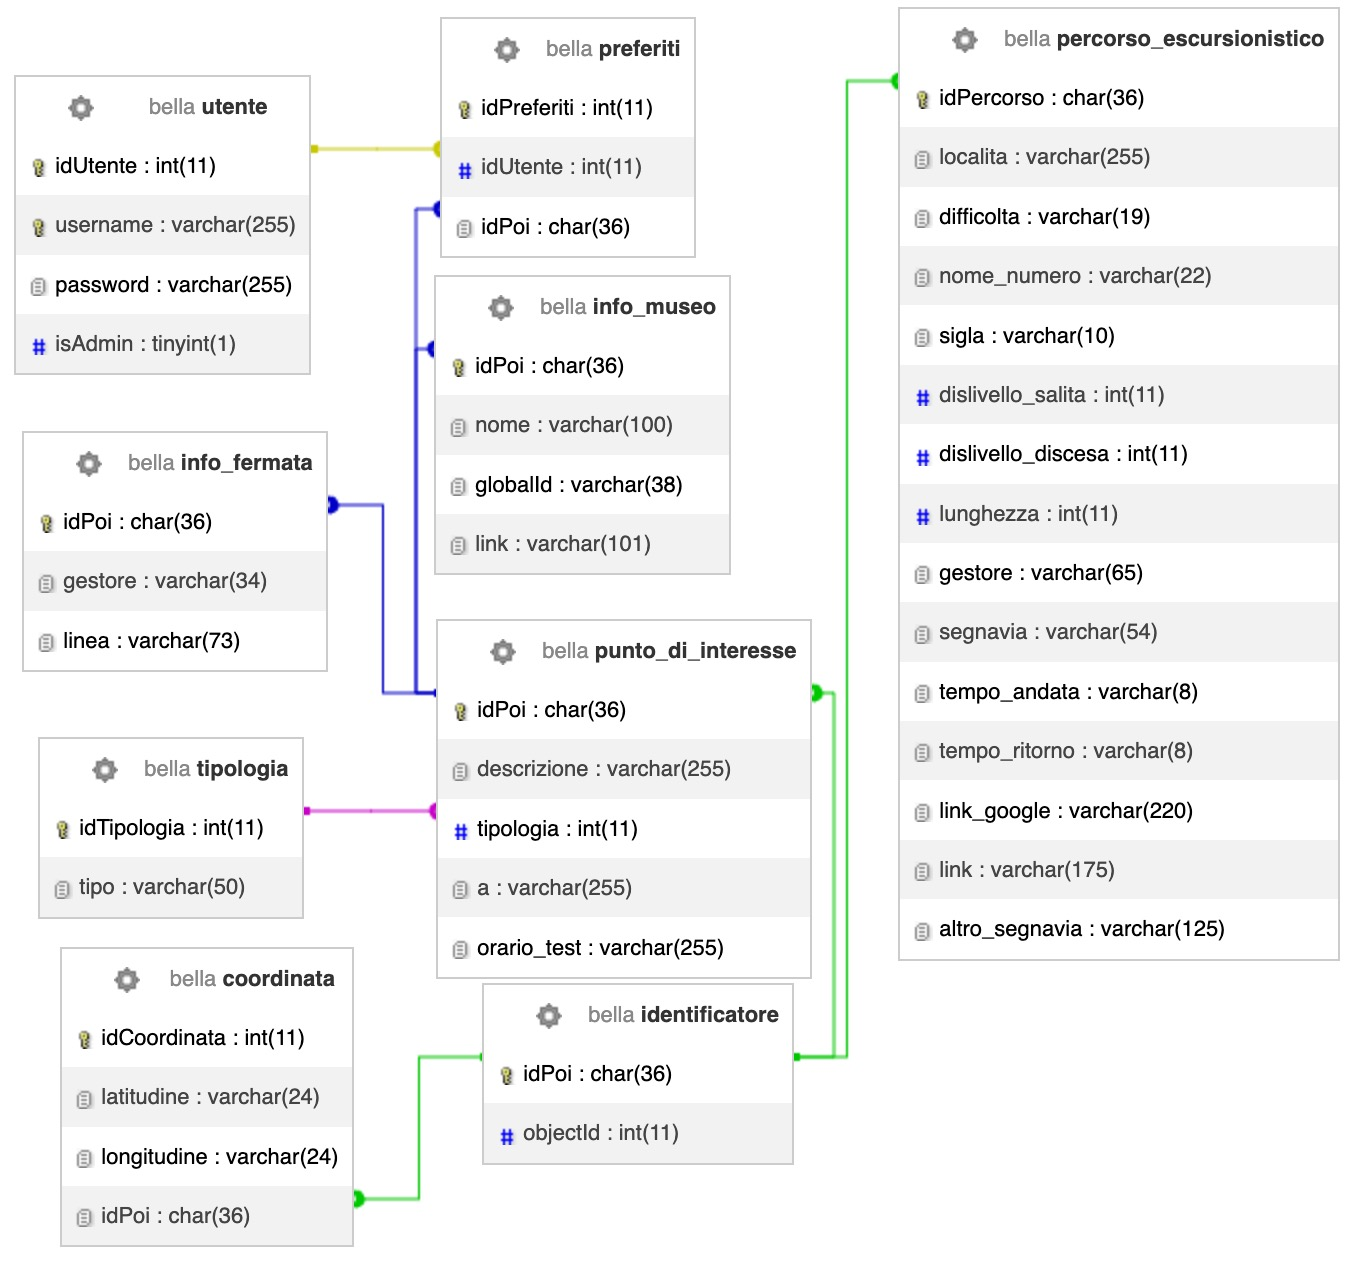
\includegraphics[width=13cm]{images/Database.jpg}
\caption[Struttura del database]{Struttura del database}\label{fig:database}
\end{center}
\end{figure}

\section{Connettere front-end e back-end}
Installato Vue.js, e creato il progetto, per connetterlo al server Apache è stato impostato un proxy, per fare in modo tale che ogni volta che venga fatta richiesta ad una cartella, tale richiesta viene inviata al server Apache ad un percorso specifico. Tutto questo è stato reso fattibile attraverso i file di impostazioni di Vue.js (figura \ref{fig:Webpack}).

\begin{figure}[h]
\begin{center}                      
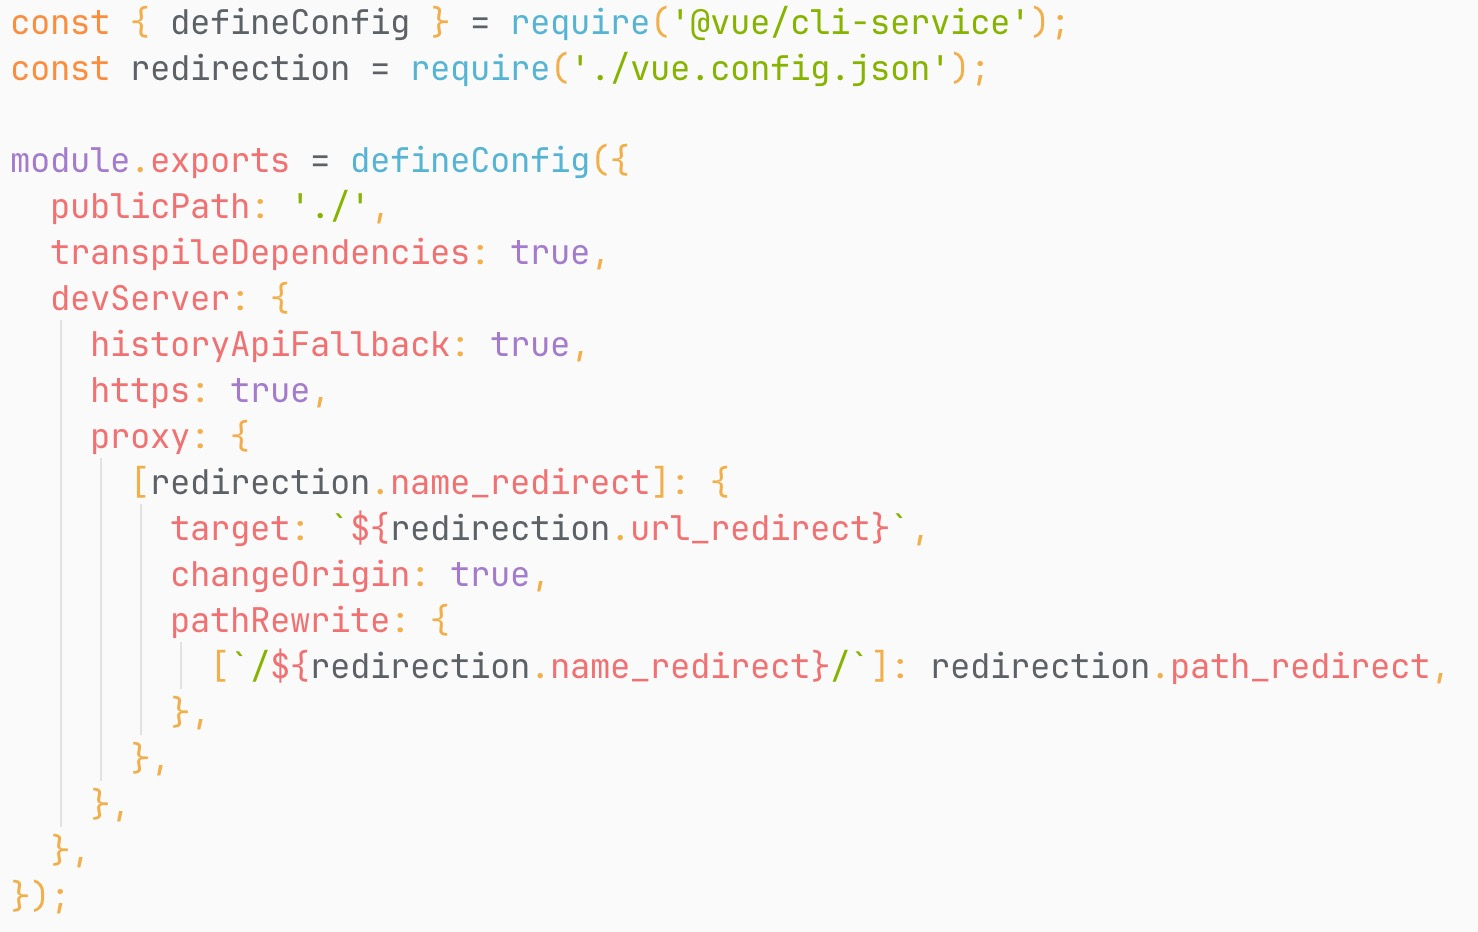
\includegraphics[width=13cm]{images/Webpack.jpg}
\caption[Impostazione web server]{Impostazioni Vue.js}\label{fig:Webpack}
\end{center}
\end{figure}

Al fine di rendere riutilizzabile questo codice, è stato creato inoltre un file \emph{JSON} chiamato ”vue.config.json” che permette di cambiare soltanto i campi principali di questo proxy senza il bisogno di riconfigurare tutto.

\subsection{Implementazione AJAX}
Al fine di fare richieste al server Apache (che successivamente interrogava il database) è stato deciso di creare una personale implementazione di AJAX anziché utilizzare librerie esterne (figura \ref{fig:ajax}).

\begin{figure}[h]
\begin{center}                      
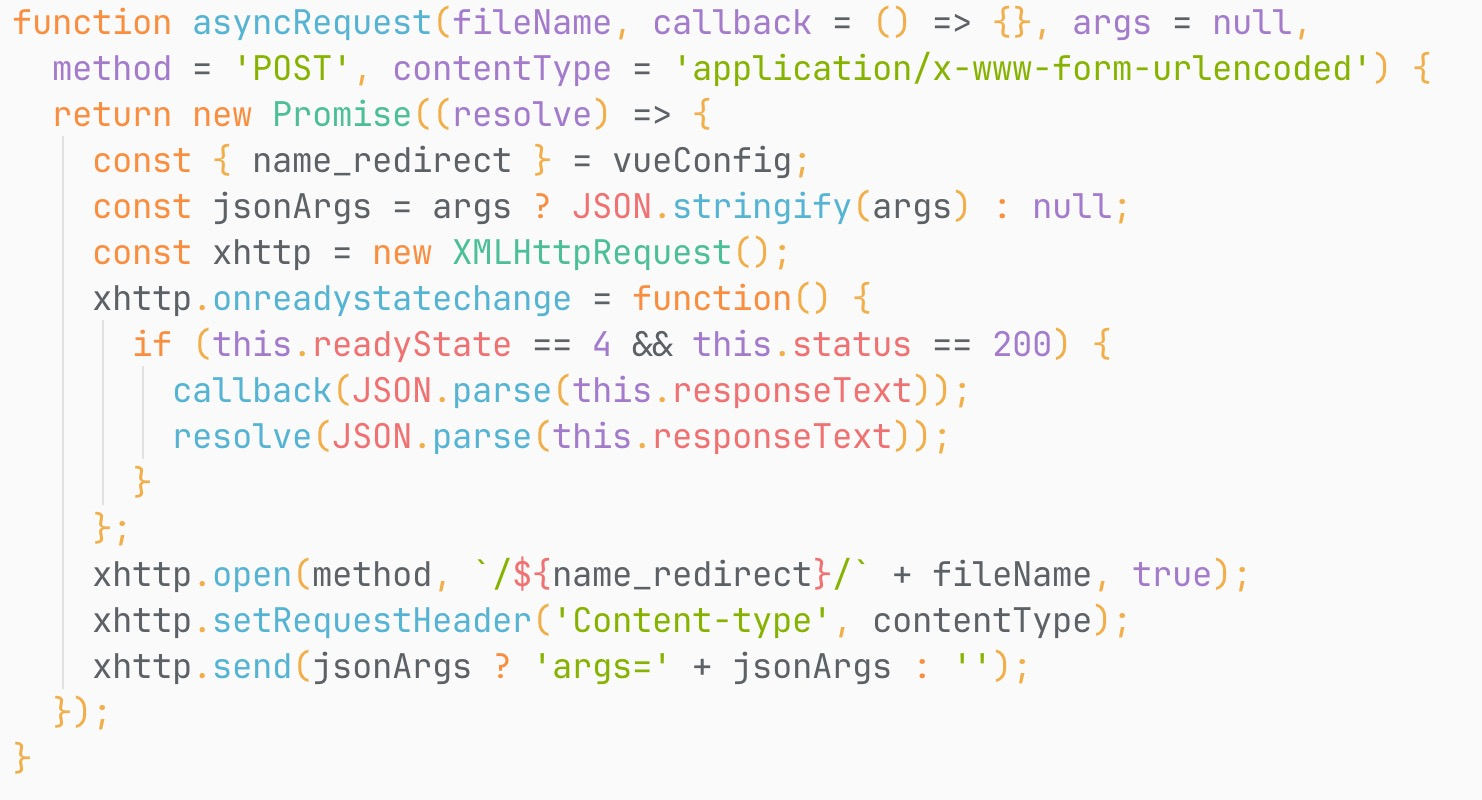
\includegraphics[width=13cm]{images/AJAX.jpg}
\caption[Implementazione di una funzione per le chiamate asincrone]{Implementazione di una funzione per le chiamate asincrone}\label{fig:ajax}
\end{center}
\end{figure}

Come parametri la funzione accetta:
\begin{itemize}
    \item Il nome del file che deve eseguire nel server Apache
    \item La funzione che deve eseguire una volta ritornata la risposta (di base inizializzata a una funzione vuota).
    \item I dati da passare (sotto forma di oggetti Javascript).
    \item Il metodo da utilizzare secondo le RESTful API (di base impostato a ”POST”).
    \item  Un parametro utilizzato per specificare il tipo di dati che stai inviando o ricevendo in una richiesta HTTP (di base impostata a ”application/x-www-form-urlencoded”). 
\end{itemize}

Dopodiché la funzione non fa altro che convertire gli oggetti Javascript da inviare in oggetti JSON. Una volta mandata la richiesta con i parametri passati e ricevuta la risposta senza alcun tipo di errore (quindi con lo stato della richiesta uguale a quattro e con la conferma della stato uguale a duecento) esegue la funzione data in input al metodo passandogli la risposta ottenuta.


\section{Popolamento Database}

Una volta configurato il proxy e creata la struttura del database rimaneva il compito di popolare il database. Come detto in precedenza i dati sono stati forniti sotto forma di file \emph{XML}, tuttavia siccome \emph{MySQL} non supporta questo tipo di file è stata creata una pagina web apposta, accessibile solo agli amministratori, che permette di svuotare e ricaricare il database, mostrando quanto tempo ha impiegato a caricare ogni tipo di punto di interesse (figura \ref{fig:Caricamento_db}).

\begin{figure}[h]
\begin{center}                      
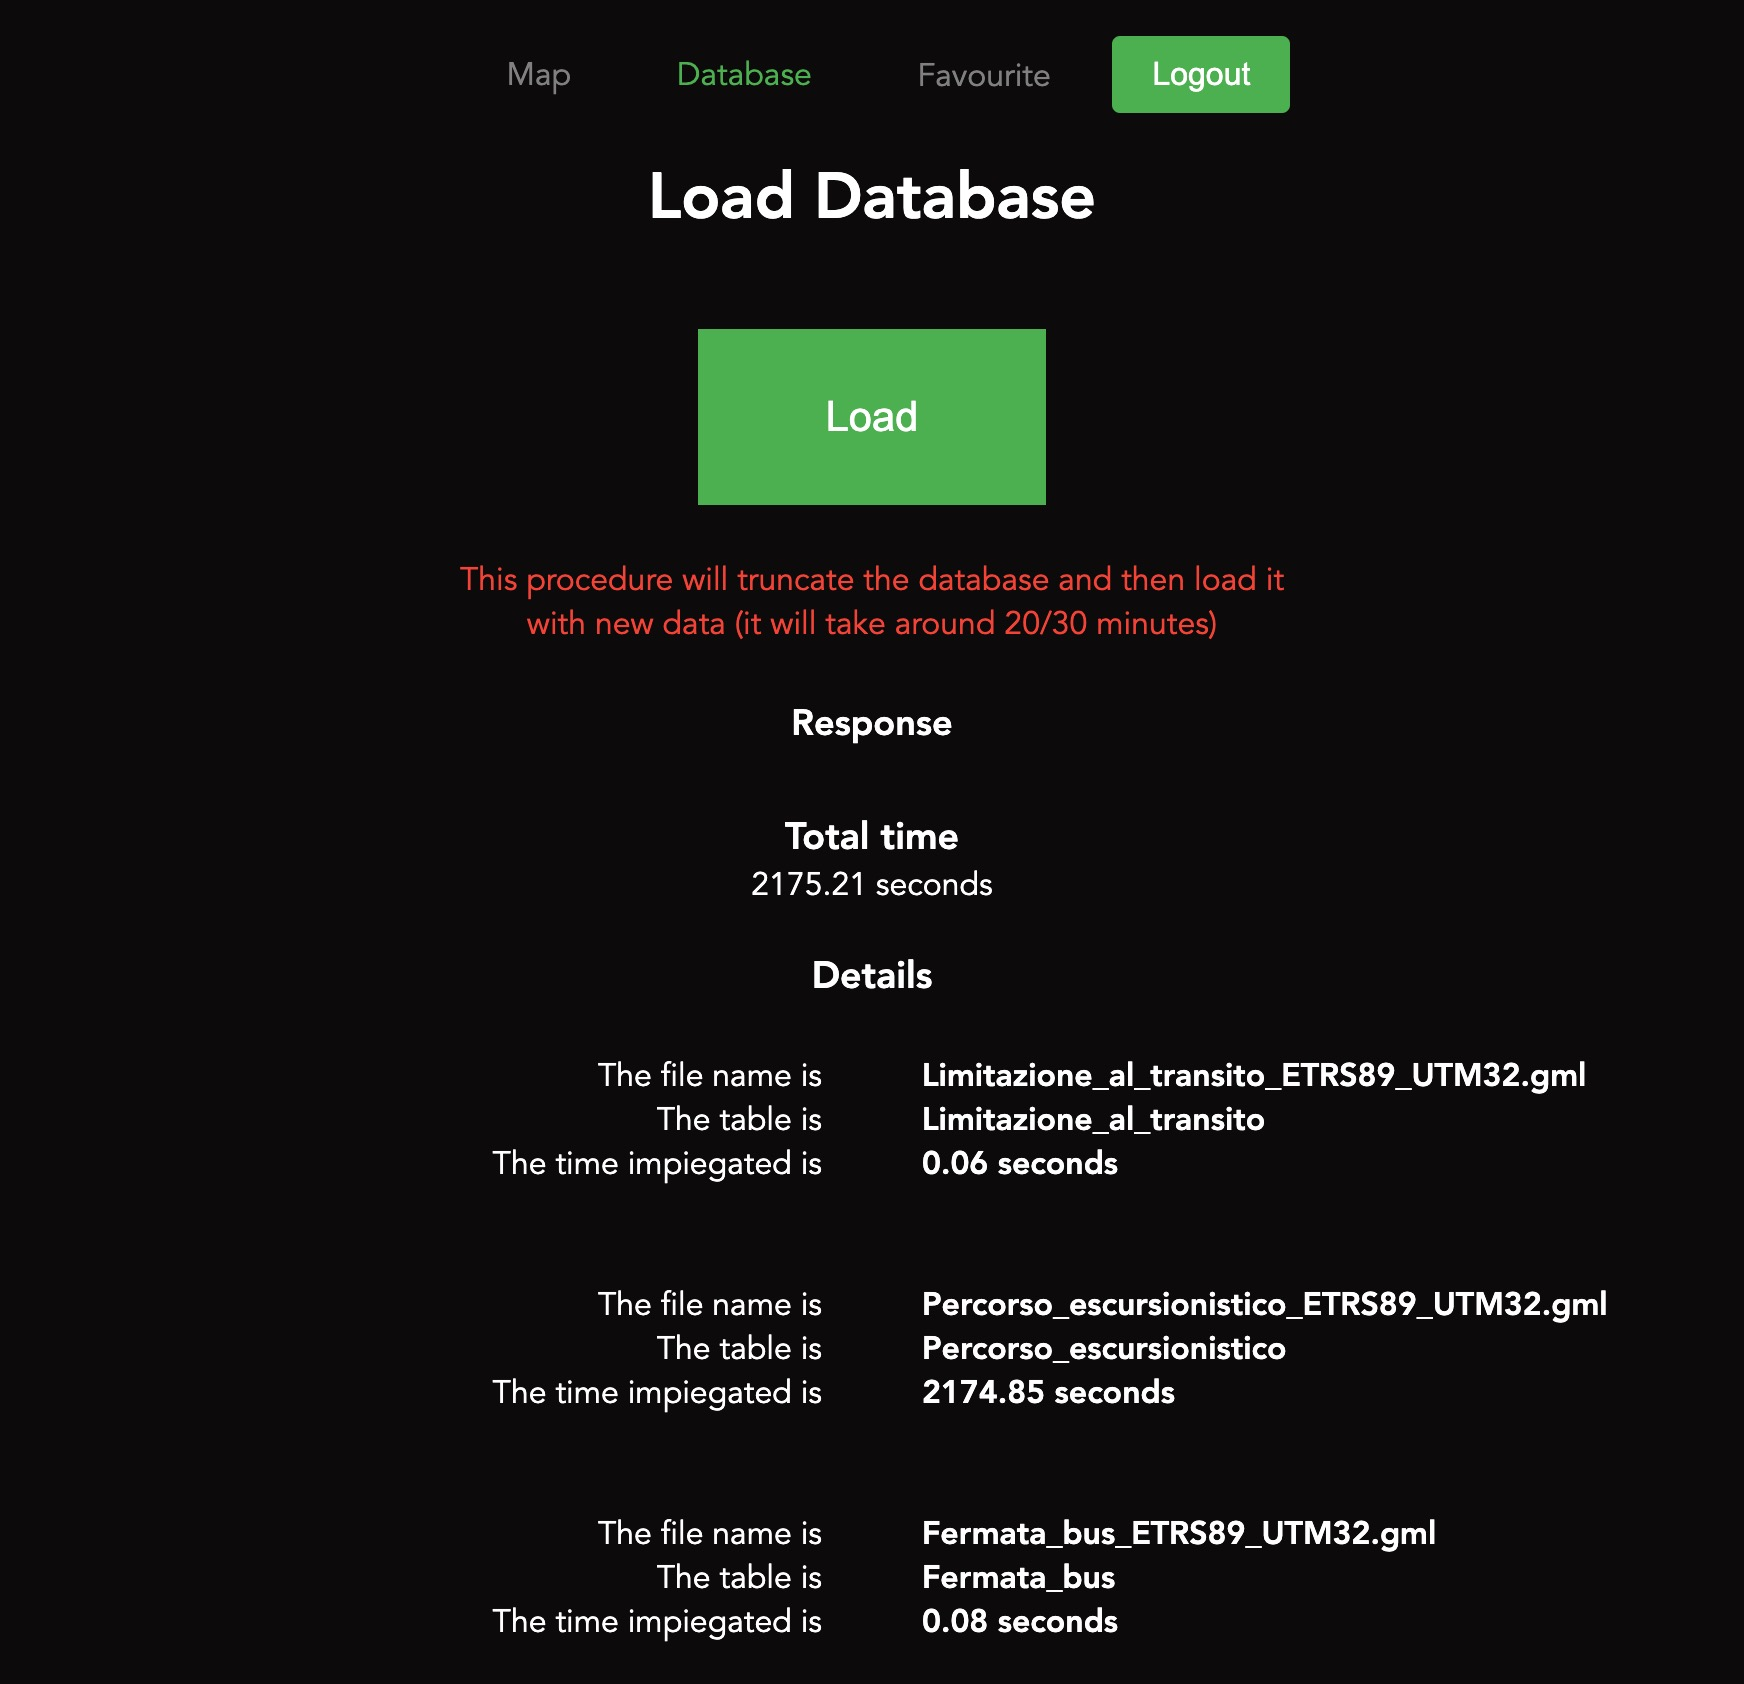
\includegraphics[width=13cm]{images/Caricamento_db.jpg}
\caption[Pagina di caricamento del database]{Pagina di caricamento del database}\label{fig:Caricamento_db}
\end{center}
\end{figure}

\section{Servizio multi pagina di Vue.js}
Una volta installato Vue-Router, un servizio di Vue.js per gestire l'indirizzamento. Dopodiché in un file sono stati creati i vari percorsi che corrispondono alle varie pagine disponibili (figura \ref{fig:route}).

\begin{figure}[h]
\begin{center}                      
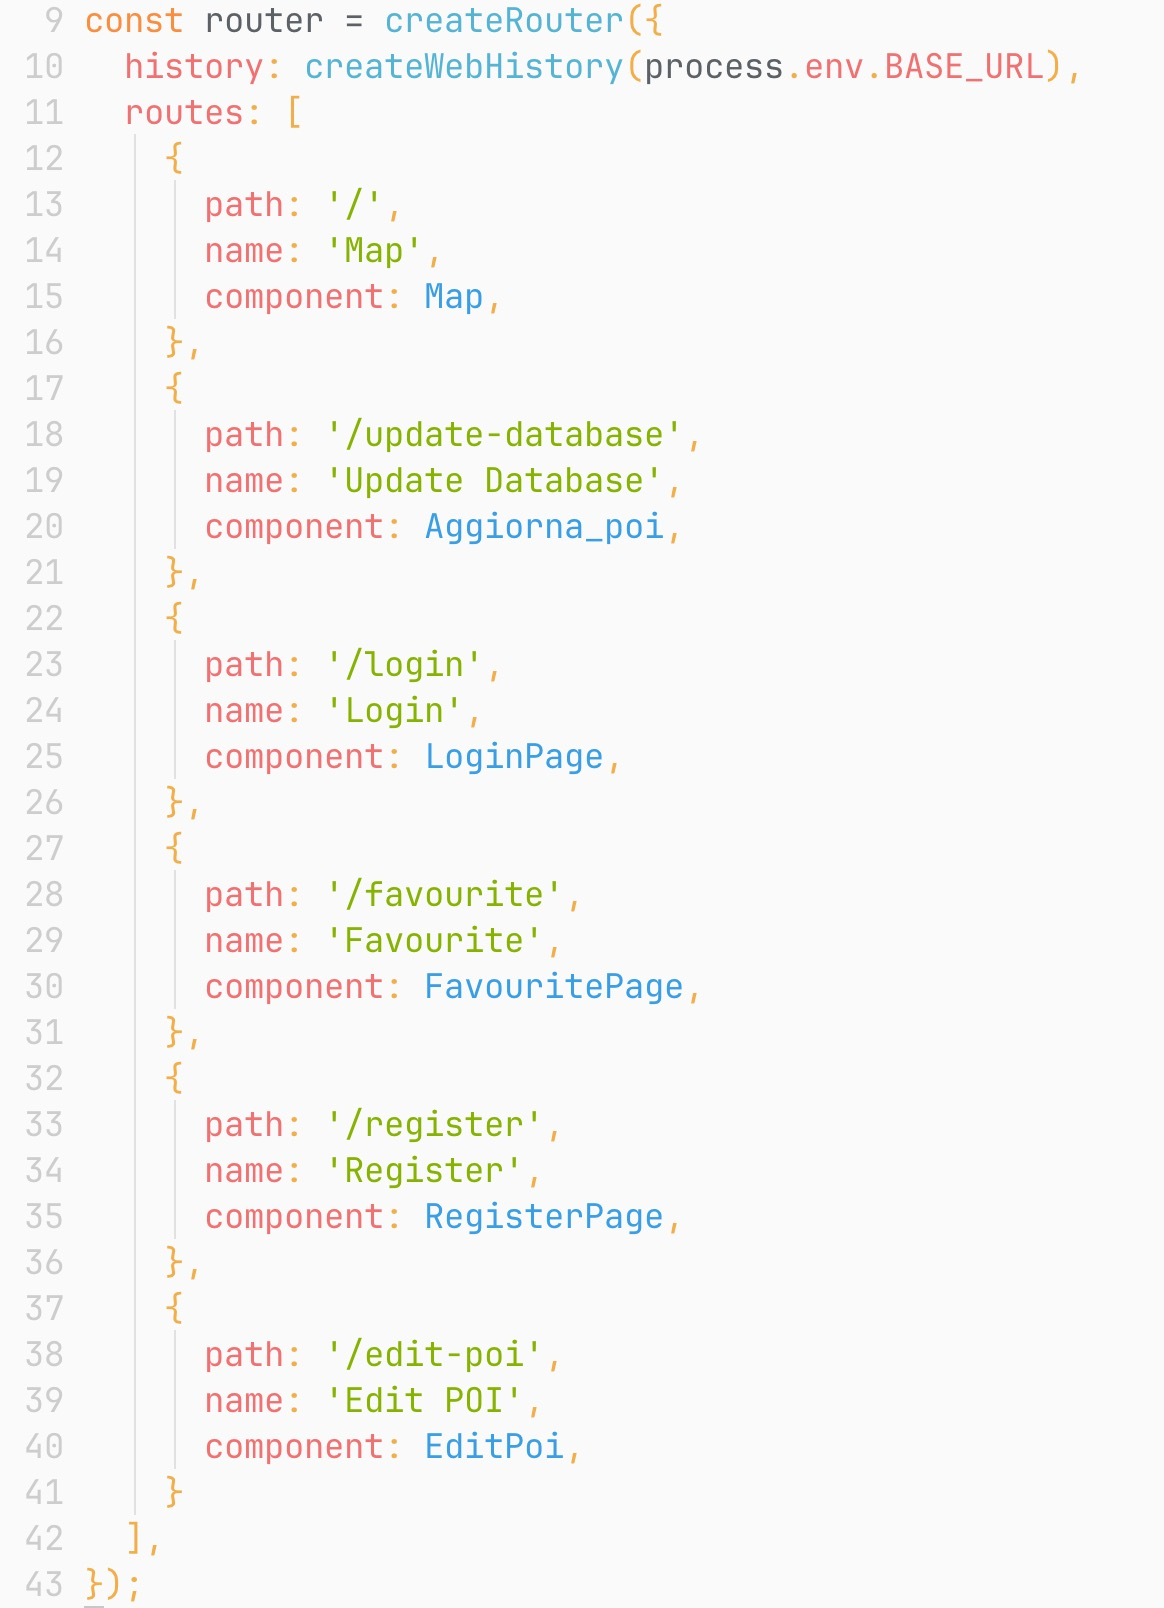
\includegraphics[width=12cm, height=14.5cm]{images/route.jpg}
\caption[Codice per impostare i vari percorsi per le pagine]{Codice per impostare i vari percorsi per le pagine}\label{fig:route}
\end{center}
\end{figure}

\section{Cura del codice}
Prima di iniziare a scrivere codice Javascript nei file Vue, ho voluto impostare uno stile di scrittura del codice utilizzando eslint al fine di avere del codice più pulito. Le regole principale impostate sono visibili in figura \ref{fig:eslint}.

\begin{figure}[h]
\begin{center}                      
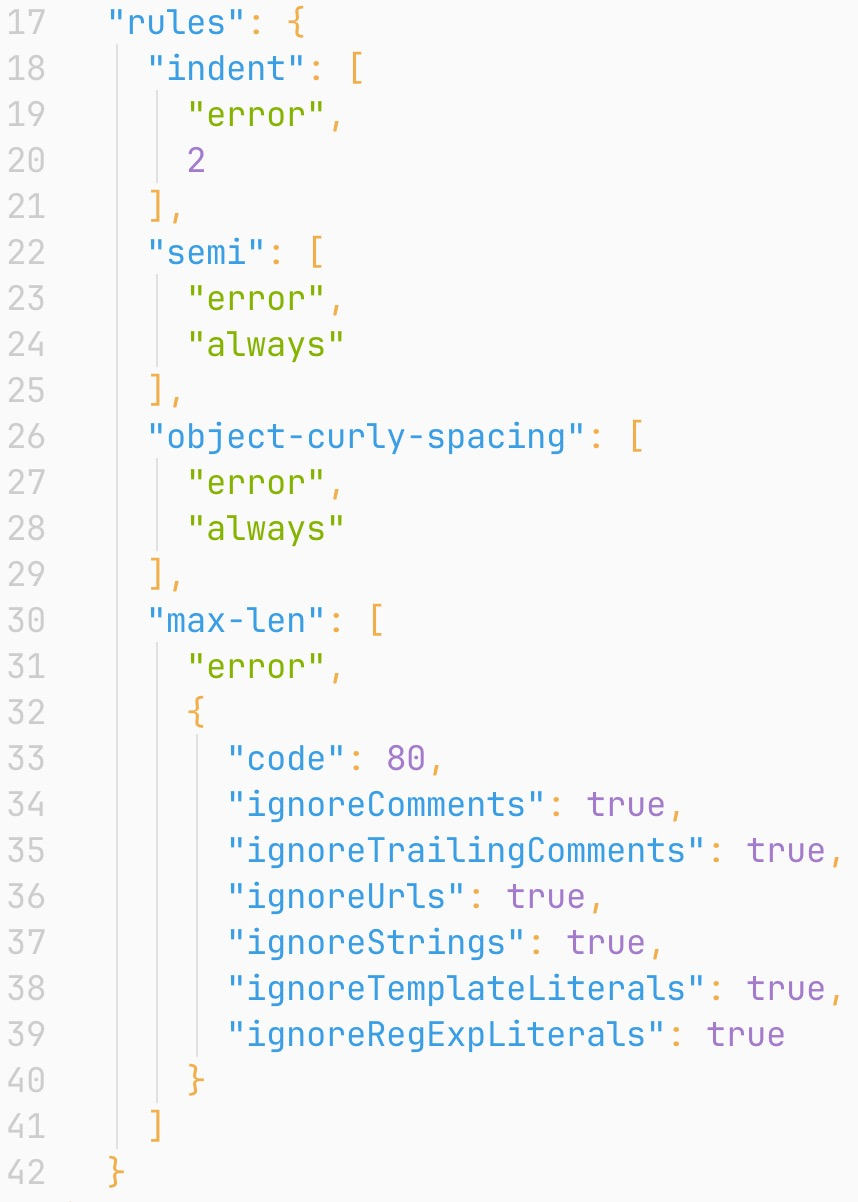
\includegraphics[width=12cm, height=13cm]{images/eslint.jpg}
\caption[Regole principale di eslint]{Regole principale di eslint}\label{fig:eslint}
\end{center}
\end{figure}

Tra queste regole, le principali sono:

\begin{itemize}
    \item La gestione dei ”tab”

    Ogni ”tab” è reso uguale a due spazi, come consigliato dalle
    \href{https://eslint.vuejs.org/}{linee guida di Vue.js}.

    \item Limitazione di caratteri su una riga

    È stato limitato il numero di caratteri su una riga fino ad un limite di 80, per assicurare maggiore leggibilità del codice.
\end{itemize}



\section{Pagina principale}
Appena caricato il database è stato possibile realizzare la pagina principale, che mostra una mappa interattiva della regione ”Emilia-Romagna” evidenziandone i percorsi escursionistici e i punti di interesse (figura \ref{fig:principale}).

\begin{figure}[h]
\begin{center}                      
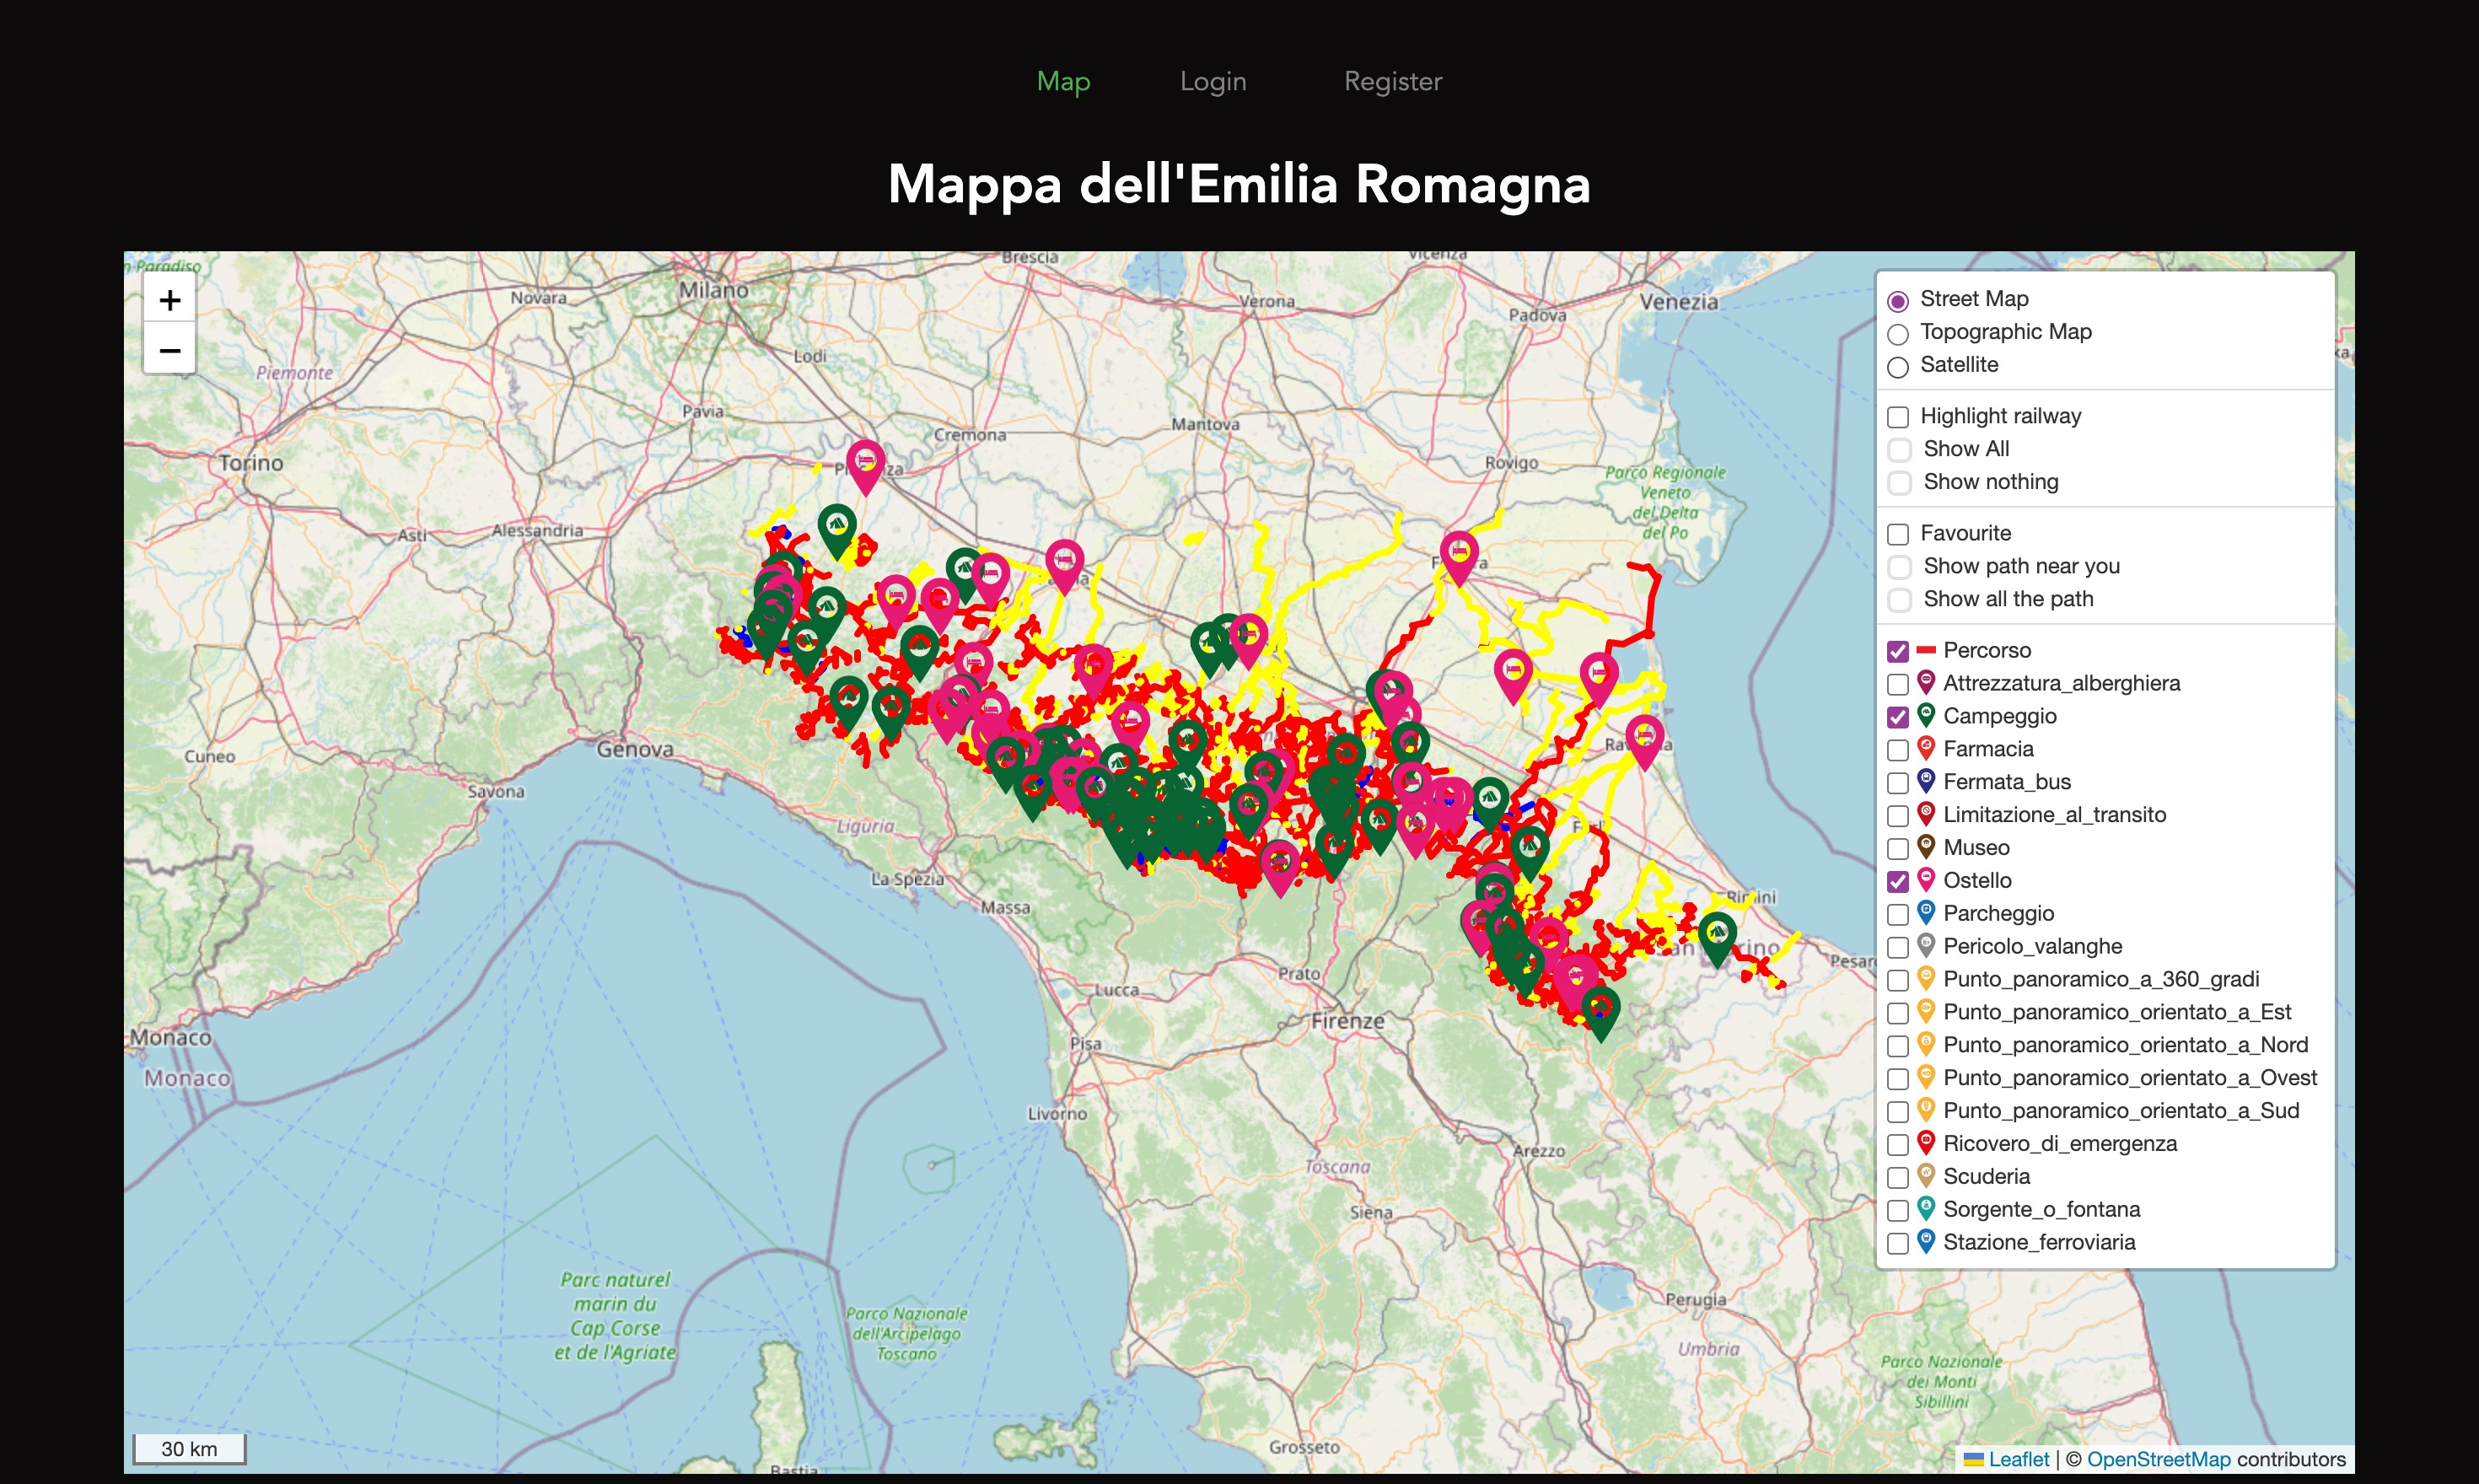
\includegraphics[width=12cm]{images/Schermata_principale.jpg}
\caption[Pagina principale]{Dimostrazione della pagina principale}\label{fig:principale}
\end{center}
\end{figure}

I vari percorsi sono colorati in base alla difficoltà:
\begin{itemize}
    \item I percorsi che sono di tipo ”E - Escursionistico” sono colorati di colore rosso
    \item I percorsi che sono di tipo ”EE - Difficile” sono colorati di colore blu
    \item I percorsi che sono di tipo ”EEA - Attrezzato” sono colorati di colore verde
    \item I percorsi che sono di tipo ”T - Turistico” sono colorati di colore giallo
\end{itemize}

In questa pagina sono presenti vari opzioni nel menù a destra.
Nella prima sezione possiamo scegliere il tipo di mappa che vogliamo mettere come sfondo, e abbiamo tre diverse opzioni:
\begin{itemize}
    \item La prima opzione è di impostare come base la cartina fisica (ed è la scelta preimpostata).
    \item La prima opzione è di impostare come base la cartina topografica.
    \item L'ultima opzione è di impostare come base la mappa satellitare.
\end{itemize}

Nella seconda sezione possiamo scegliere se mostrare tutti i punti di interesse, nasconderli tutti o mettere in risalto i percorsi ferroviari (figura \ref{fig:railway}).

\begin{figure}[h]
\begin{center}                      
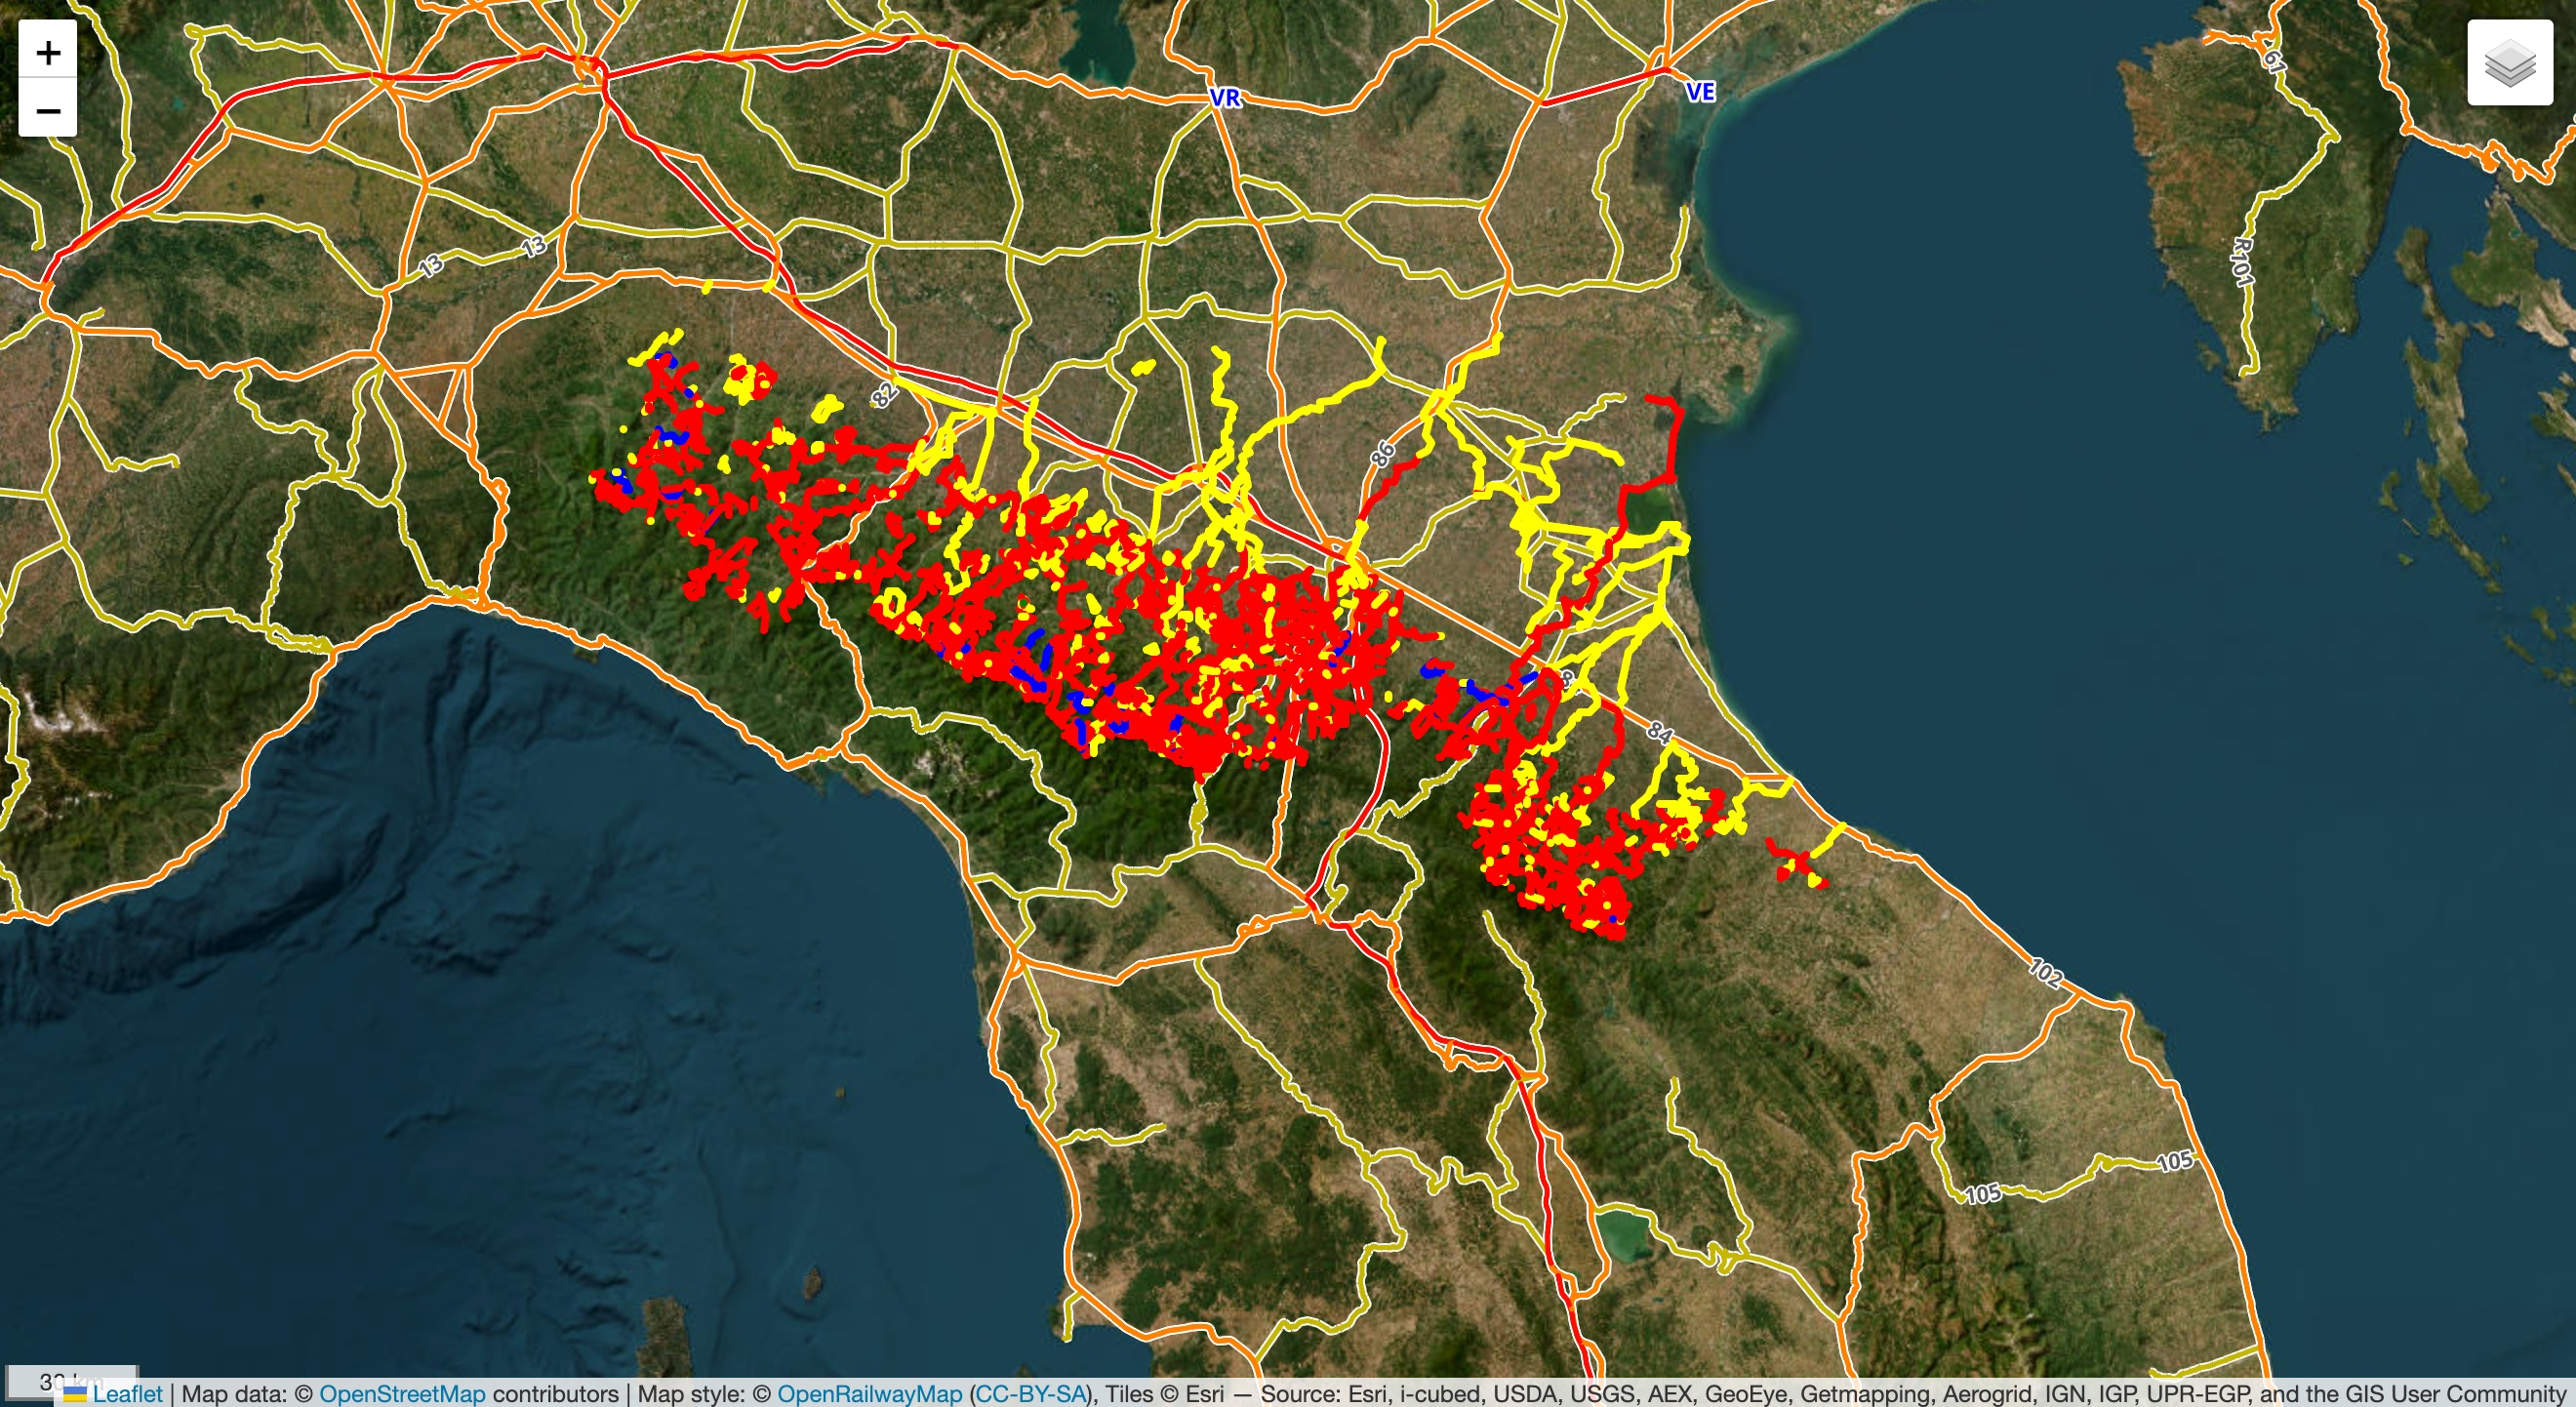
\includegraphics[width=0.7\textwidth]{images/Railway.jpg}
\caption[Mappa satellitare con i percorsi ferroviari evidenziati]{Mappa satellitare con i percorsi ferroviari evidenziati}\label{fig:railway}
\end{center}
\end{figure}

Nella terza sezione del menù possiamo scegliere se mostrare i punti di interesse aggiunti come preferiti (solo nel caso in cui l'utente abbia effettuato la registrazione e l'accesso), se mostrare tutti i percorsi della regione o se mostrare solo i percorsi vicini alla posizione dell'utente.

Infine nell'ultima sezione è possibile scegliere quali punti di interesse mostrare e nascondere.

\section{Geo localizzazione}

L'applicazione permette inoltre di mostrare solamente i  percorsi nelle vicinanze in un raggio di 40km. Per calcolare i quali percorsi mostrare viene utilizzata la formula di Haversine che ci permette di calcolare in modo efficiente le distanze geografiche sulla superficie terrestre~\cite{Haversine}.

La formula di Haversine è espressa come segue:

\begin{align*}
a &= \sin^2\left(\frac{\Delta\phi}{2}\right) + \cos(\phi_1) \cdot \cos(\phi_2) \cdot \sin^2\left(\frac{\Delta\lambda}{2}\right) \\
c &= 2 \cdot \text{atan2}\left(\sqrt{a}, \sqrt{1-a}\right) \\
d &= R \cdot c
\end{align*}

Dove:
\begin{align*}
\Delta\phi & \text{ è la differenza di latitudine tra i due punti.} \\
\Delta\lambda & \text{ è la differenza di longitudine tra i due punti.} \\
\phi_1 & \text{ è la latitudine del primo punto.} \\
\phi_2 & \text{ è la latitudine del secondo punto.} \\
R & \text{ è il raggio della Terra (approssimativamente 6,371 km).}
\end{align*}

I valori ottenuti sono:
\begin{itemize}
    \item \emph{a} che è un valore che viene utilizzato successivamente per calcolare altre componenti.

    \item \emph{c} che rappresenta l'angolo calcolato usando il valore $\alpha$ e la funzione atan2. Questo angolo è utilizzato per calcolare la distanza sulla superficie terrestre tra i due punti.

    \item \emph{d} che rappresenta la distanza sulla superficie terrestre tra i due punti, misurata in unità di lunghezza specificate dal raggio terrestre $R$. Questa è la distanza effettiva tra i due punti che stai cercando di calcolare.
\end{itemize}

Quindi infine viene controllato il valore \emph{d} che rappresenta la distanza tra le coordinate del percorso che si vuole mostrare e le coordinate della posizione dell'utente(figura \ref{fig:vicina}).

\begin{figure}[h]
\begin{center}                      
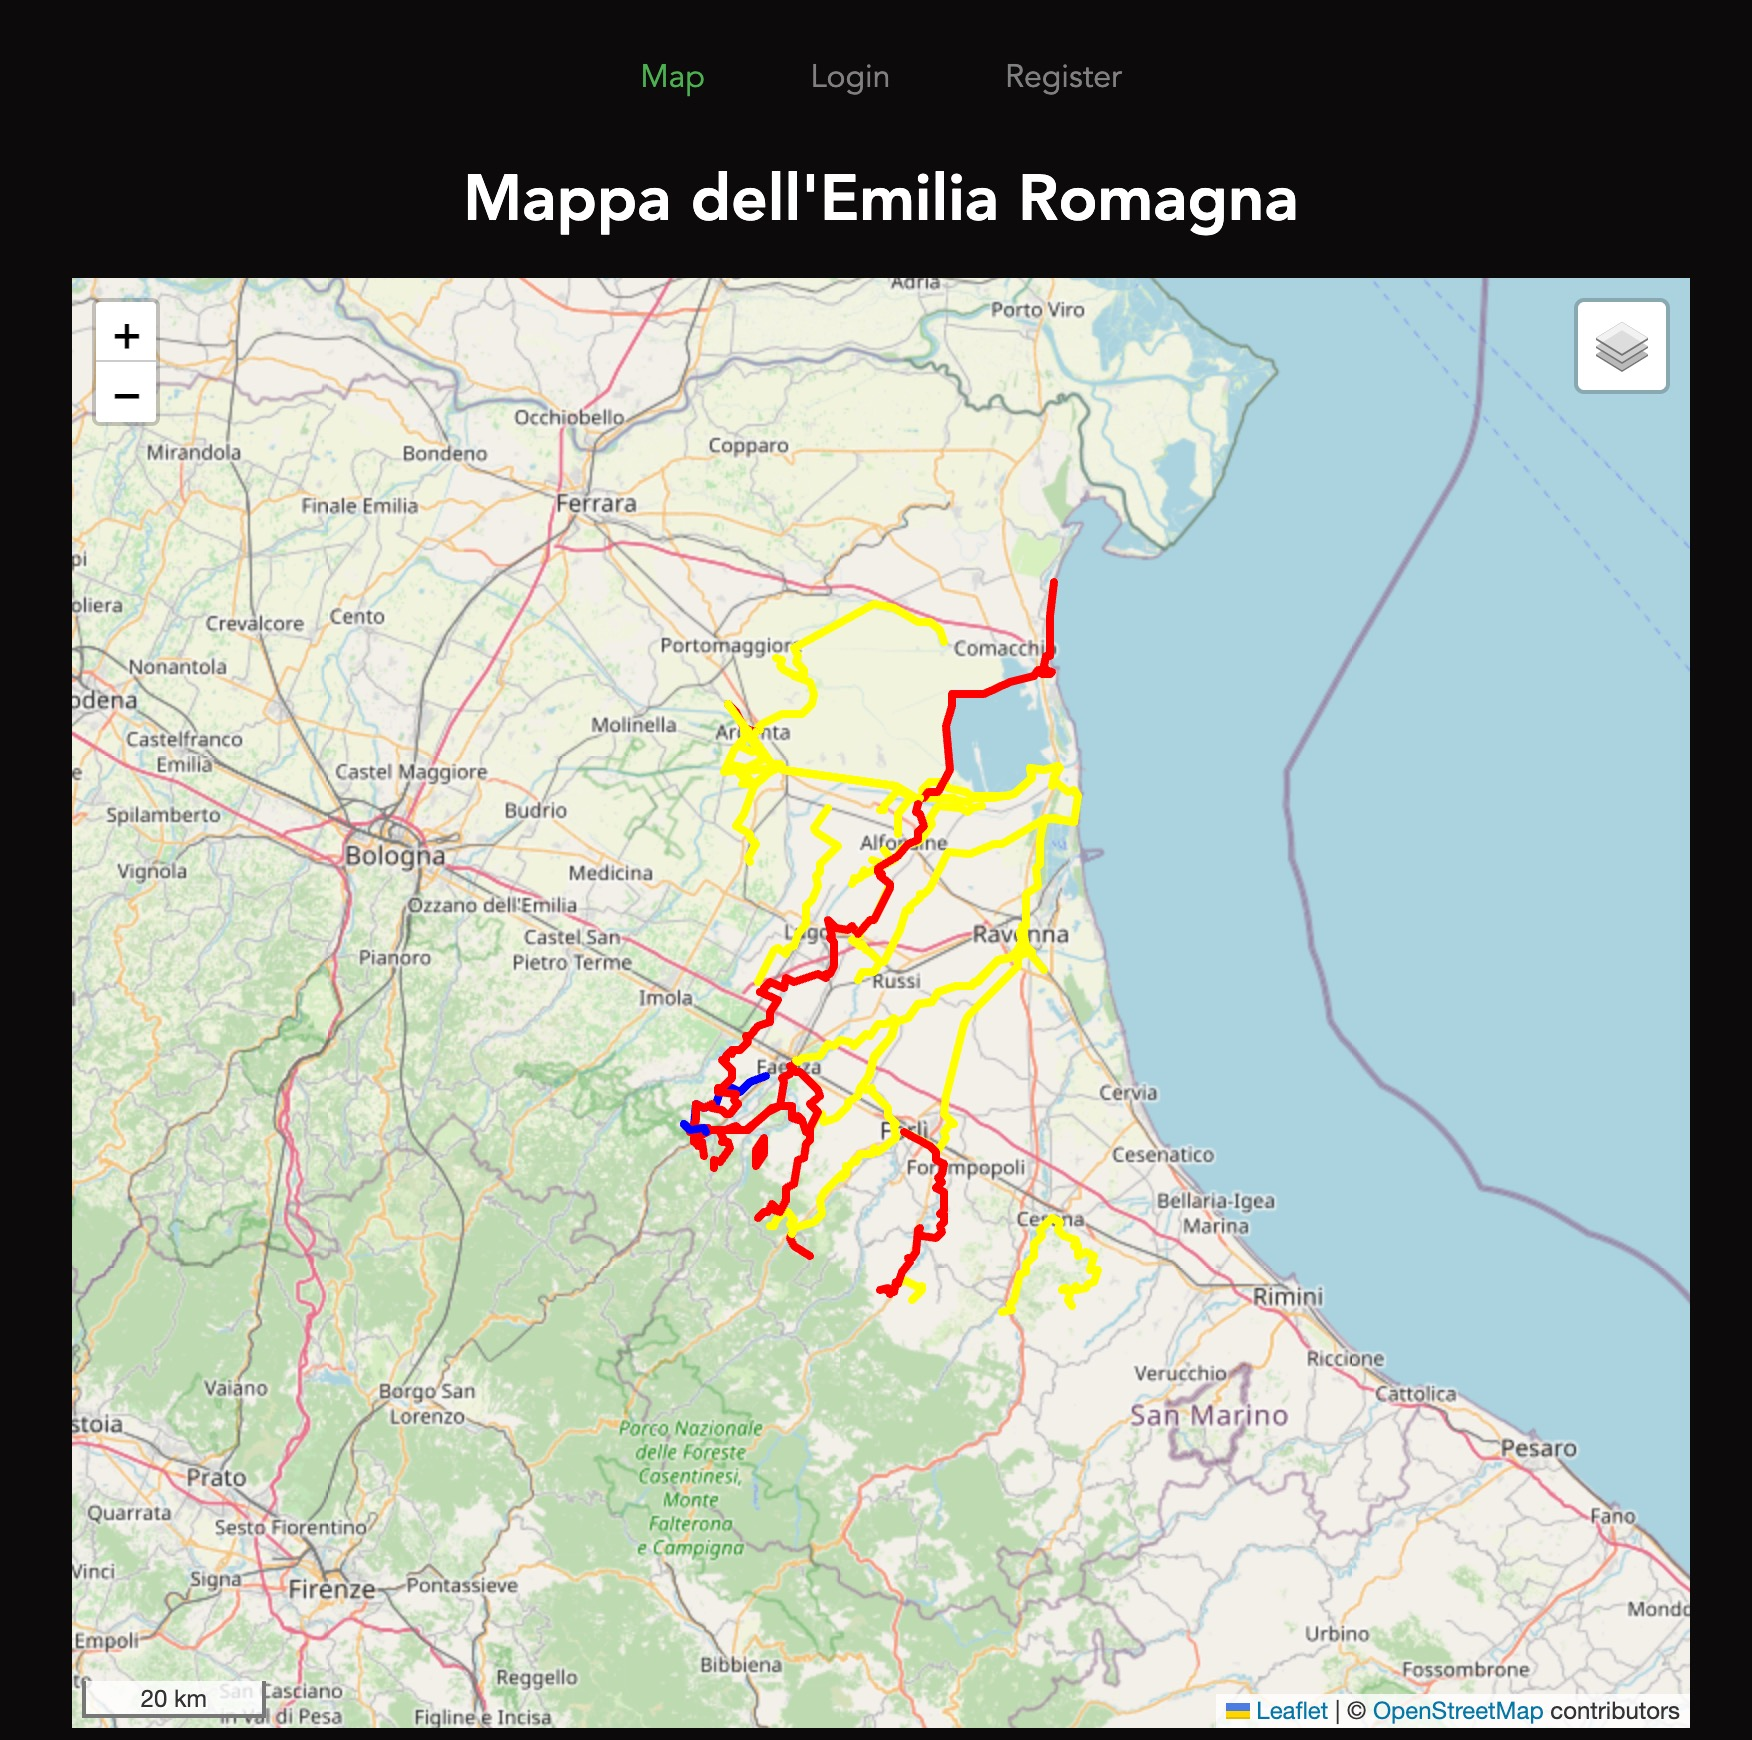
\includegraphics[width=0.7\textwidth]{images/Mappa_vicina.jpg}
\caption[Dimostrazione funzionamento mappa]{Dimostrazione cartina con percorsi vicini all'utente (test effettuato nel centro della città di Ravenna)}\label{fig:vicina}
\end{center}
\end{figure}


\section{Informazioni sui percorsi}
È possibile ottenere informazioni su ogni singolo percorso escursionistico cliccandoci sopra, come dimostrato in figura \ref{fig:info}.

\begin{figure}[h]
\begin{center}                      
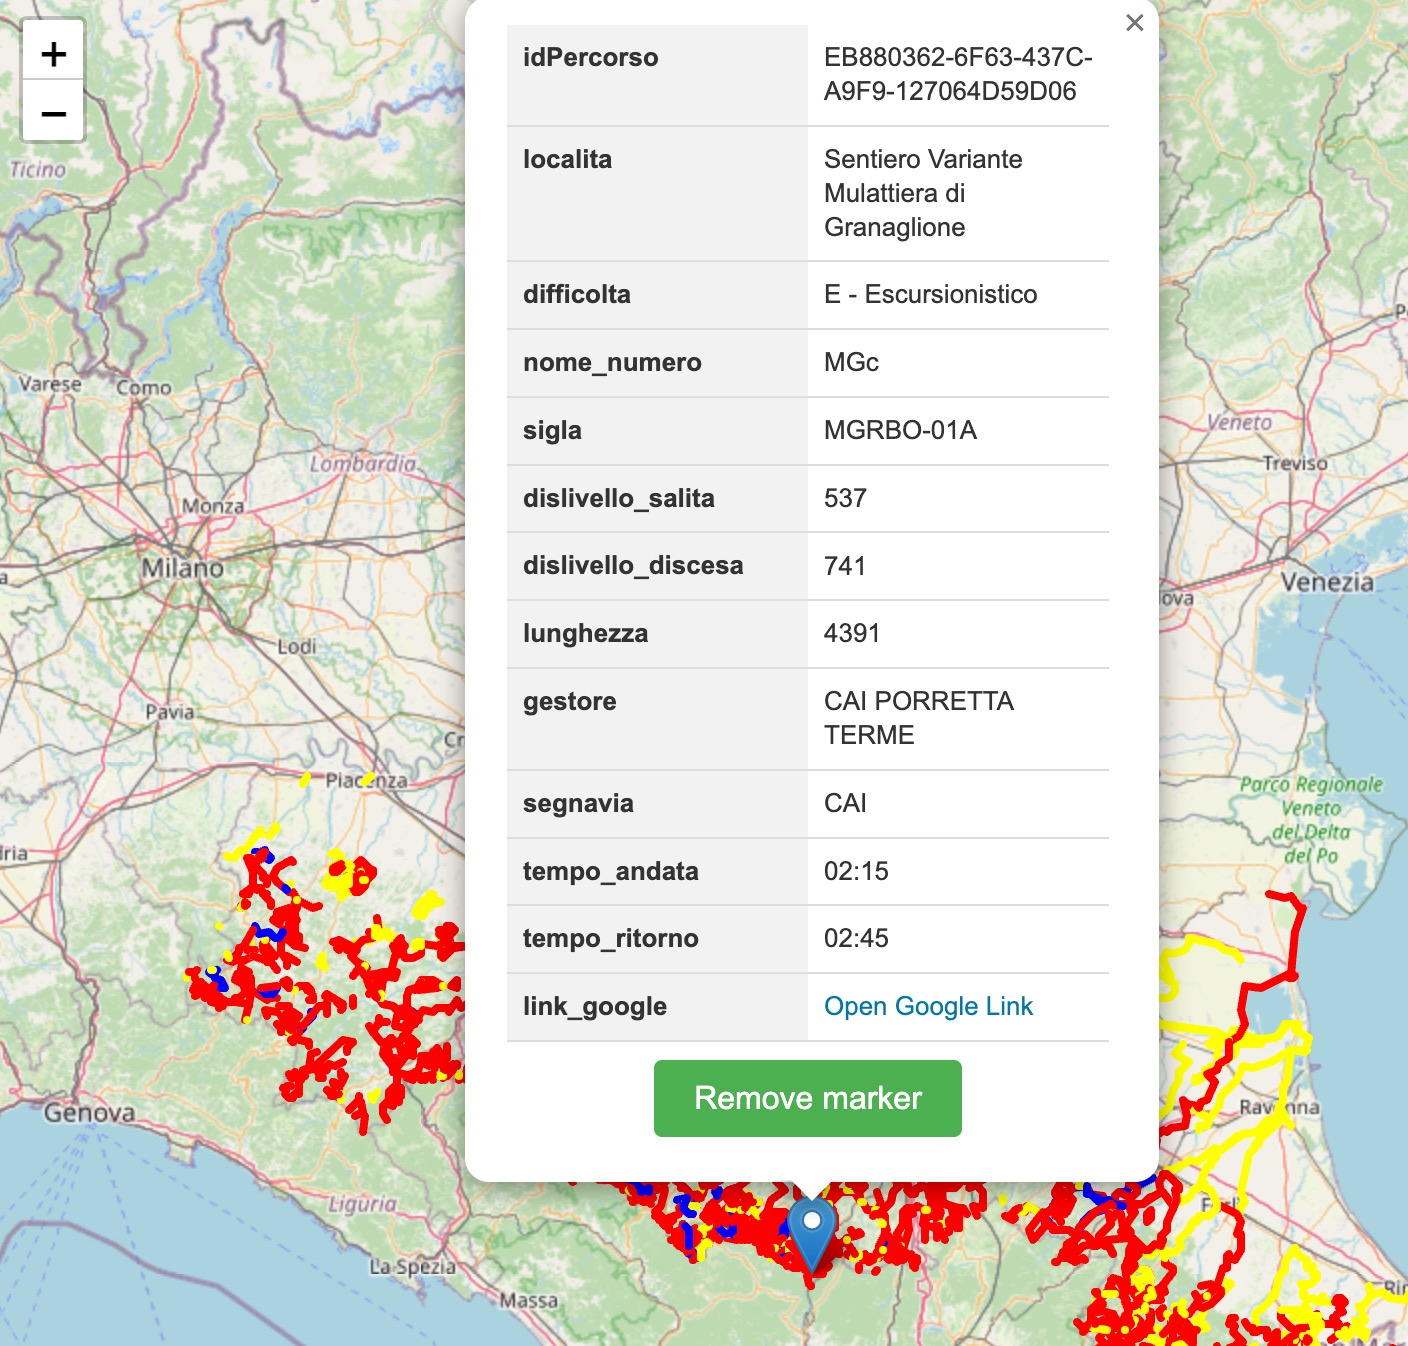
\includegraphics[width=12cm]{images/Informazioni percorso.jpg}
\caption[Dimostrazione informazioni mappa]{Informazioni di un percorso}\label{fig:info}
\end{center}
\end{figure}

\section{Registrazione e accesso}
È possibile registrarsi (figura \ref{fig:registrazione}) e eseguire l'accesso (figura \ref{fig:login}) al fine di aggiungere informazioni sui punti di interesse o di creare una lista di punti di interesse preferiti.

\begin{figure}[h]
    \centering
    \begin{minipage}{0.40\textwidth}
        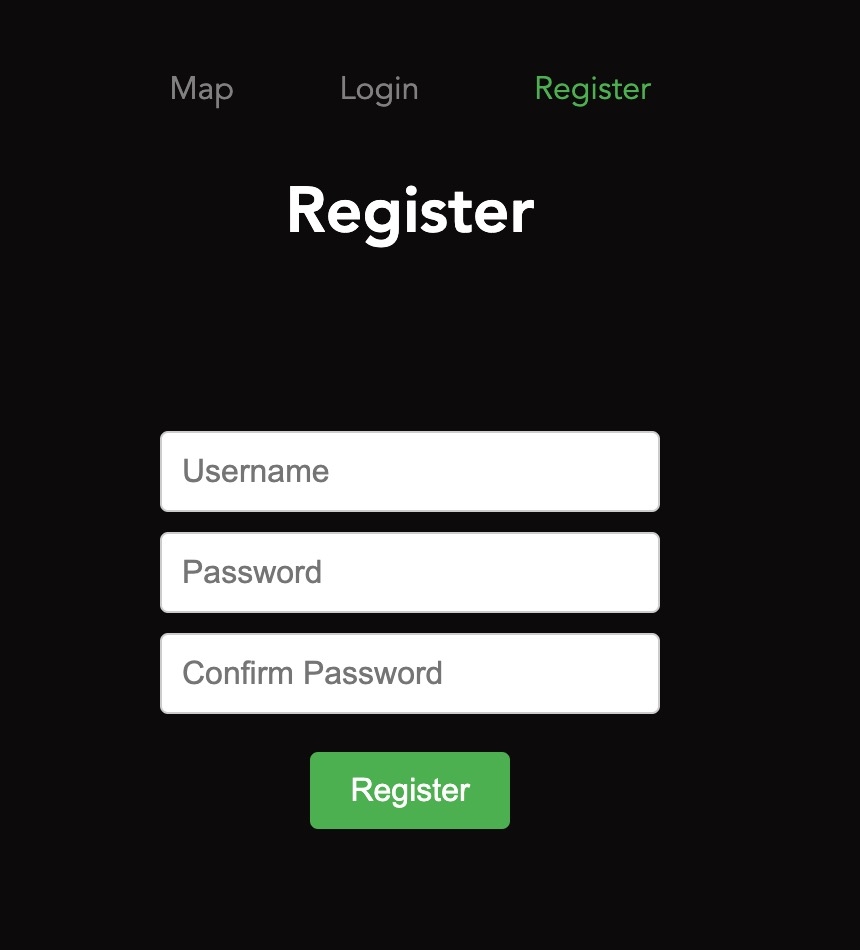
\includegraphics[width=\textwidth]{images/Registrazione.jpg}
        \caption[Pagina di registrazione]{Pagina di registrazione}
        \label{fig:registrazione}
    \end{minipage}

    \vspace{0.6cm}

    \begin{minipage}{0.40\textwidth}
        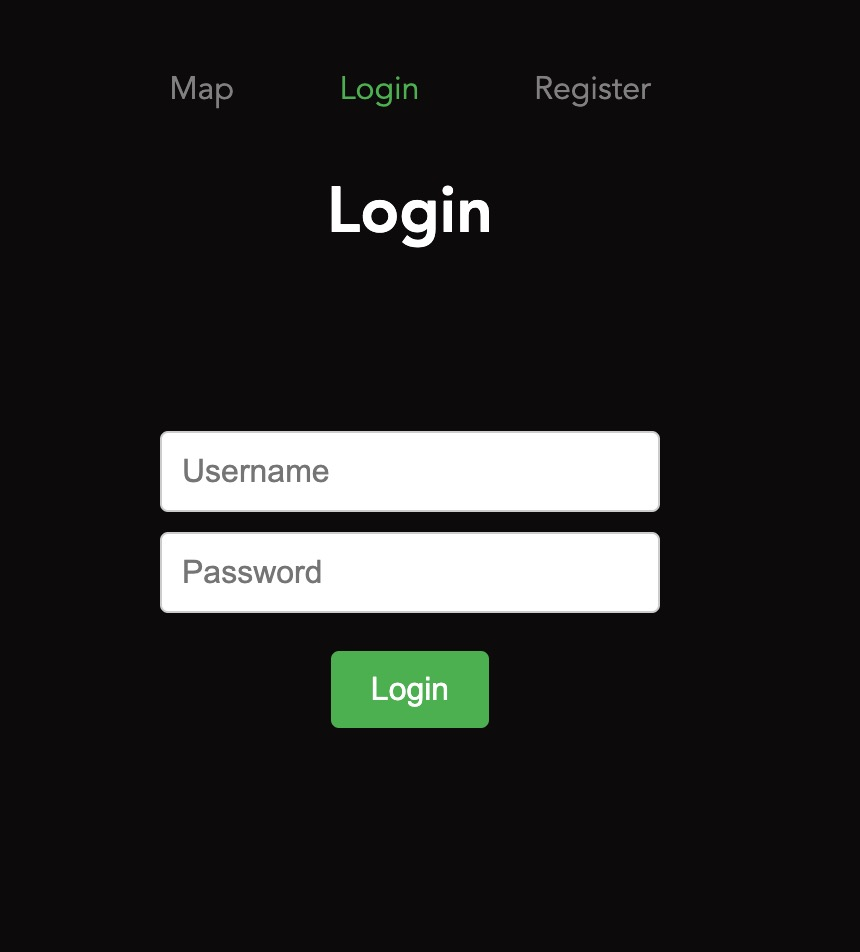
\includegraphics[width=\textwidth]{images/Login.jpg}
        \caption[Pagina per effettuare l'accesso]{Pagina per effettuare l'accesso}
        \label{fig:login}
    \end{minipage}
\end{figure}

\section{Informazioni sui punti di interesse}
Nel caso in cui l'utente clicchi su un punto di interesse è possibile vedere le sue informazioni. Se l'utente ha effettuato l'accesso è inoltre possibile aggiungere altre informazioni e aggiungere il punto nella lista dei punti preferiti (figura \ref{fig:info_punto}).

\begin{figure}[h]
\begin{center} 
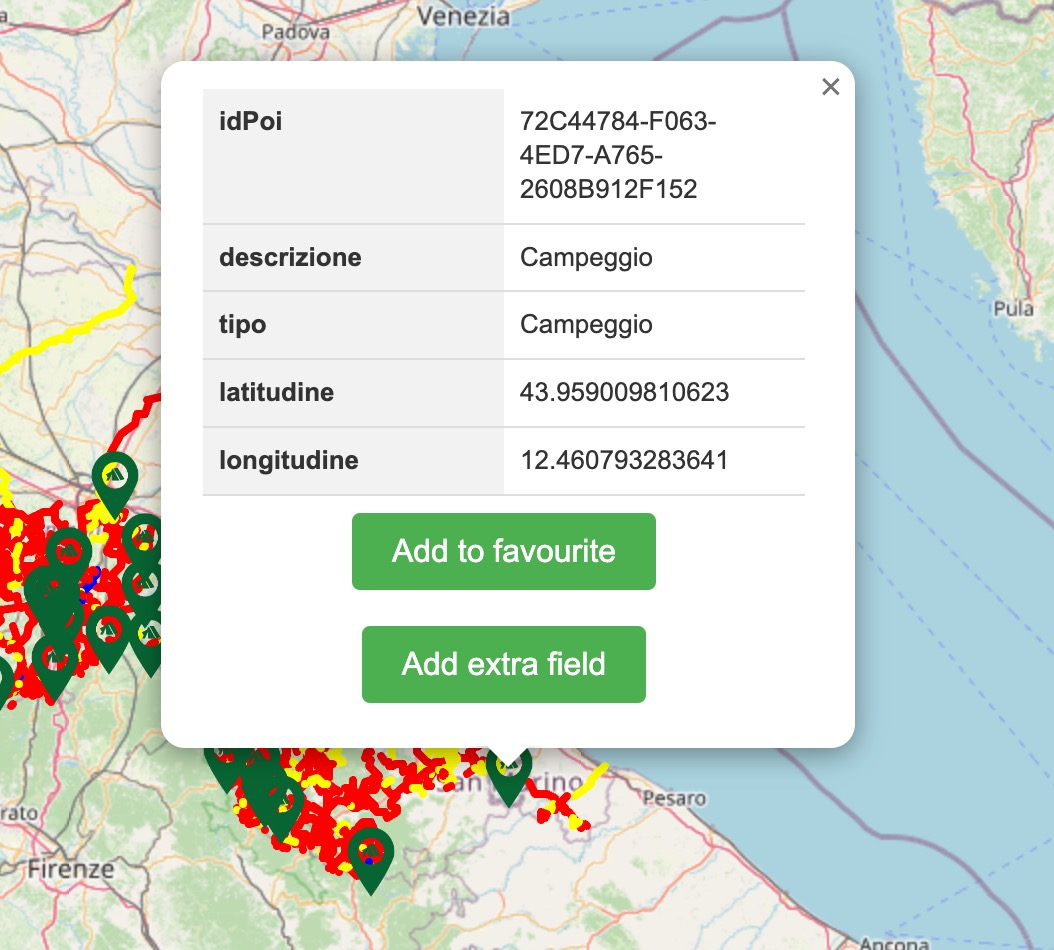
\includegraphics[width=12cm]{images/Info punto.jpg}
\caption[Informazioni di un percorso]{Informazioni di un percorso}\label{fig:info_punto}
\end{center}
\end{figure}

\section{Pagina dei preferiti}

Una volta che l'utente ha eseguito l'accesso e ha aggiunto dei punti di interesse nella sua lista dei preferiti, è possibile vedere una pagina (figura \ref{fig:preferiti}) che mostri tutte le informazioni su questi punti, insieme alla possibilità di filtrarli.

\begin{figure}[h]
\begin{center} 
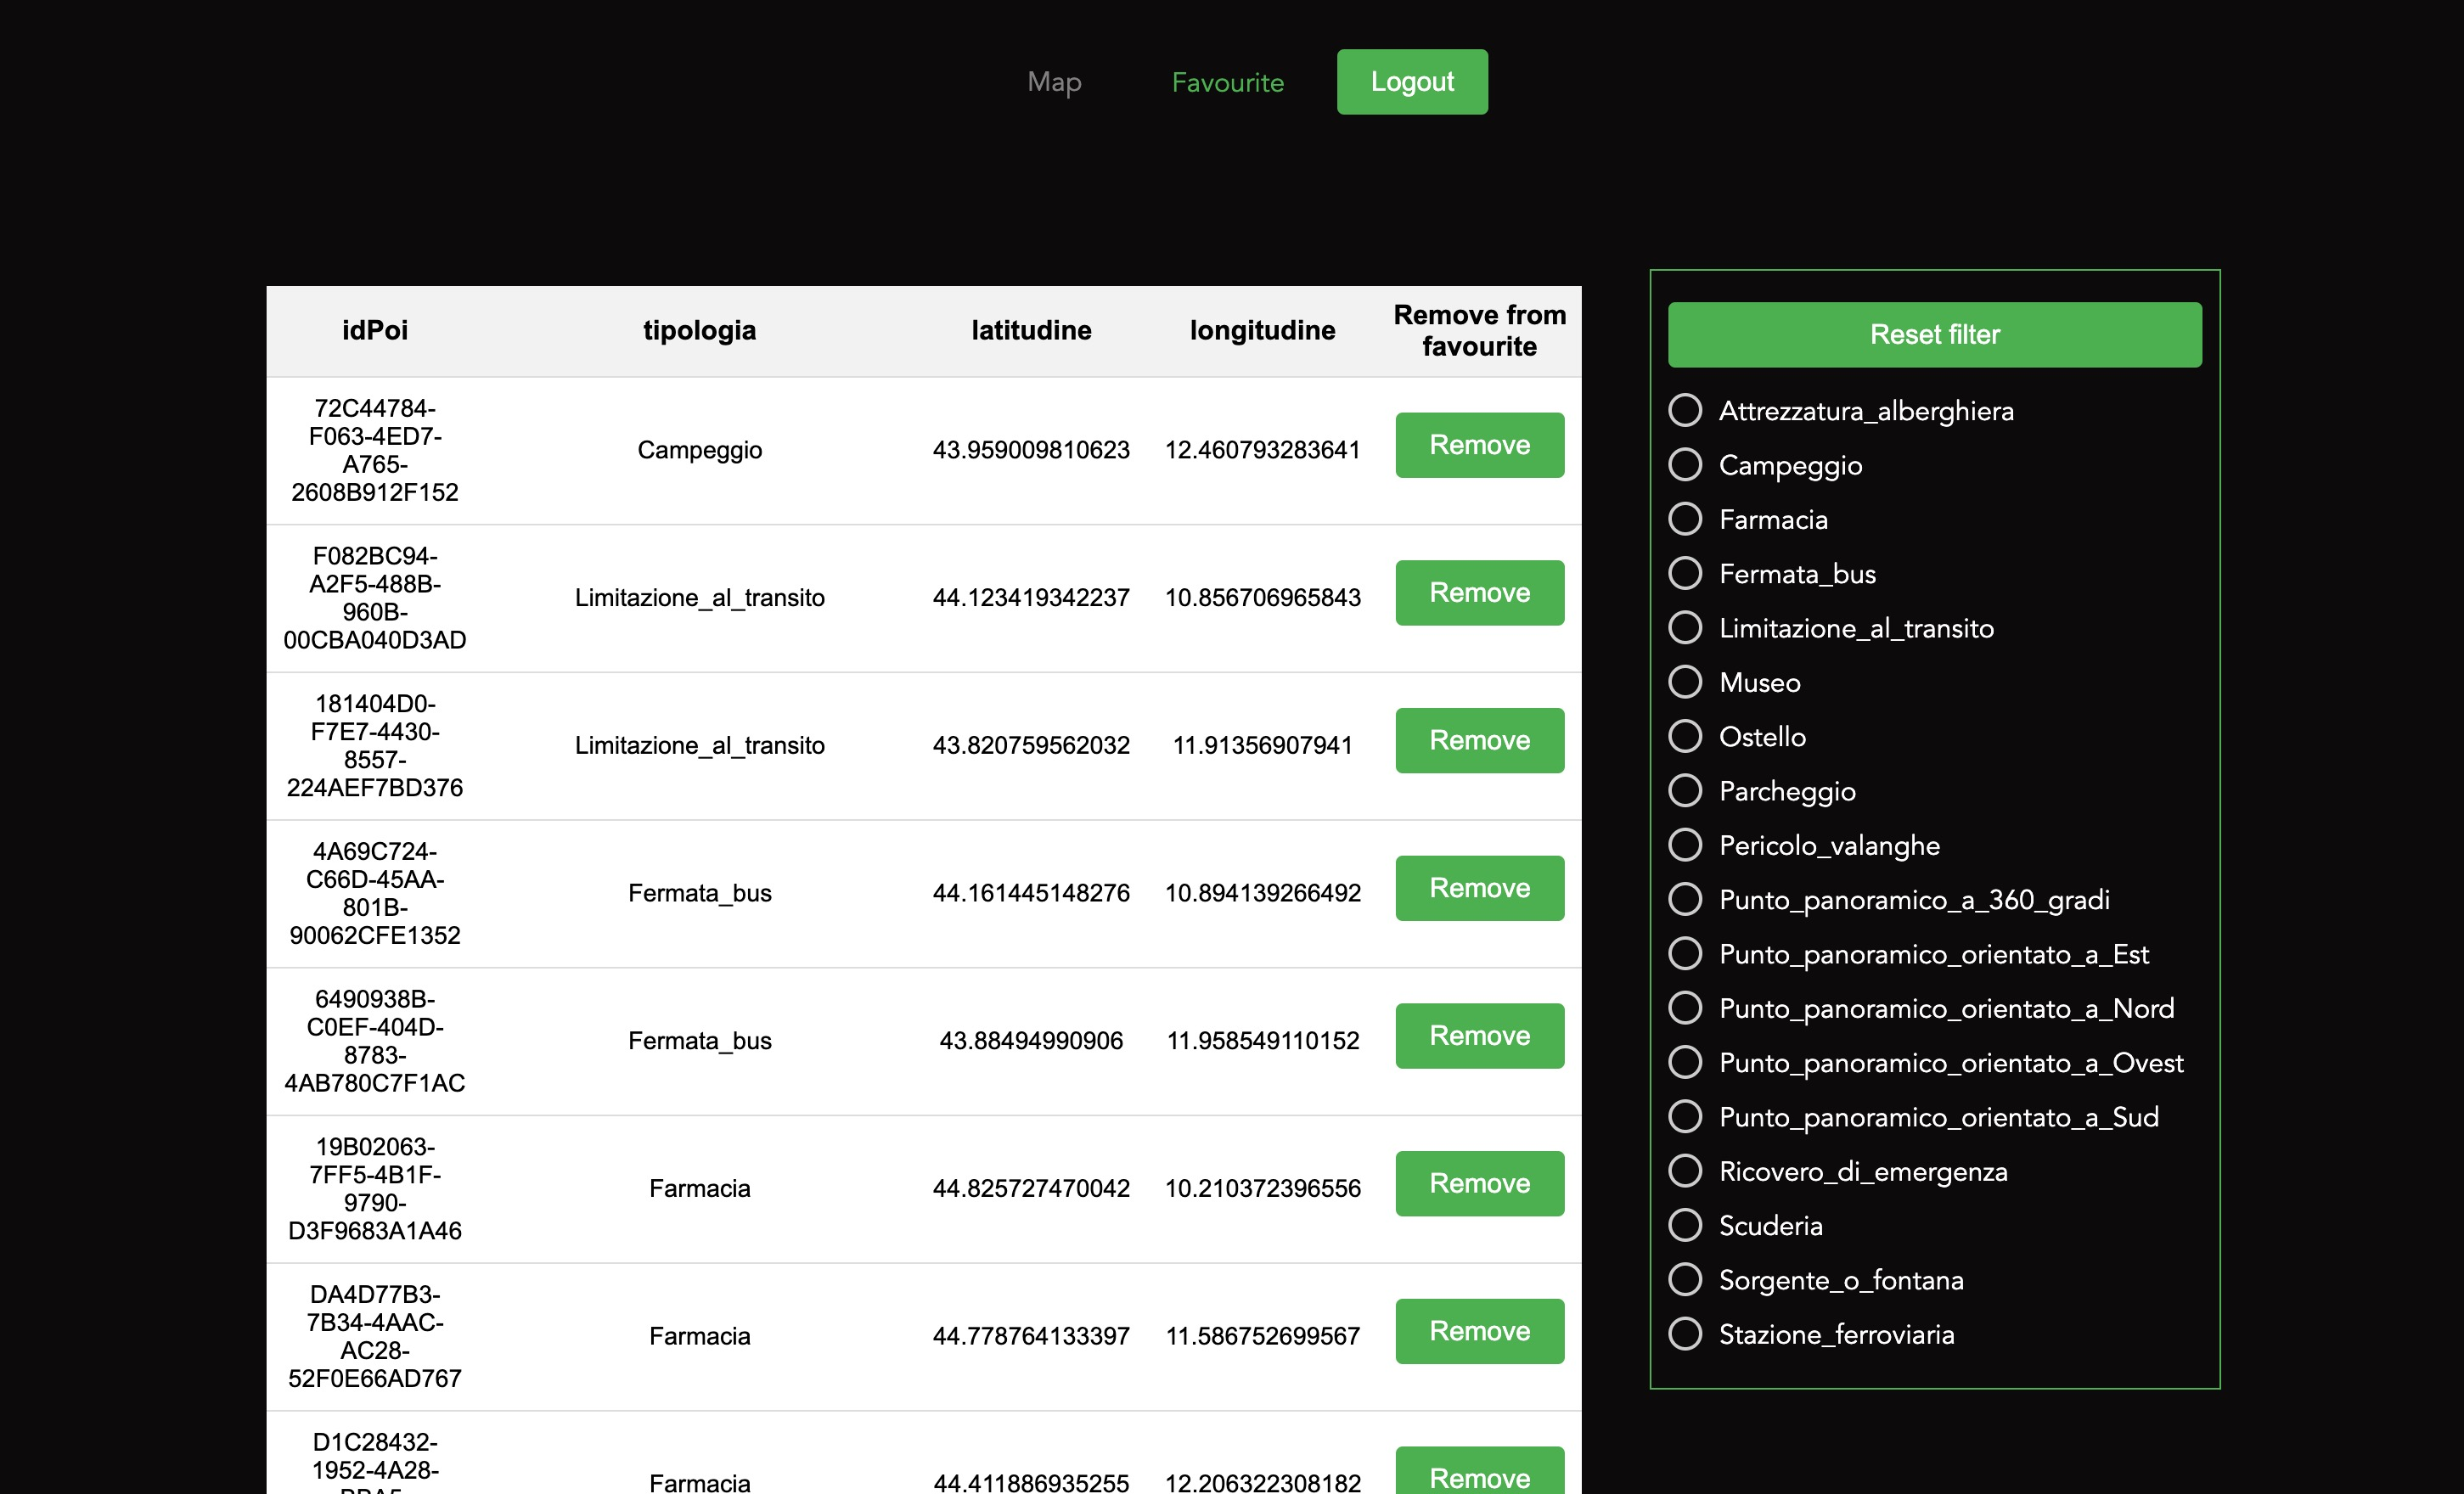
\includegraphics[width=13cm]{images/Favourite page.jpg}
\caption[Pagina dei preferiti]{Pagina dei preferiti}\label{fig:preferiti}
\end{center}
\end{figure}


Da questa pagina è possibile vedere l'identificativo di ogni punto, che tipo di punto di interesse sia e le sue coordinate. Inoltre questa pagina permette di rimuovere ogni elemento dalla lista dei preferiti.

\section{Aggiungere informazioni ai punti}
Una volta che l'utente è registrato può aggiungere informazioni su ogni punto di interesse (come visibile in figura \ref{fig:info_punto}). La pagina da cui eseguire questa operazione appare come raffigurato in figura \ref{fig:extra_field}.

\begin{figure}[h]
\begin{center} 
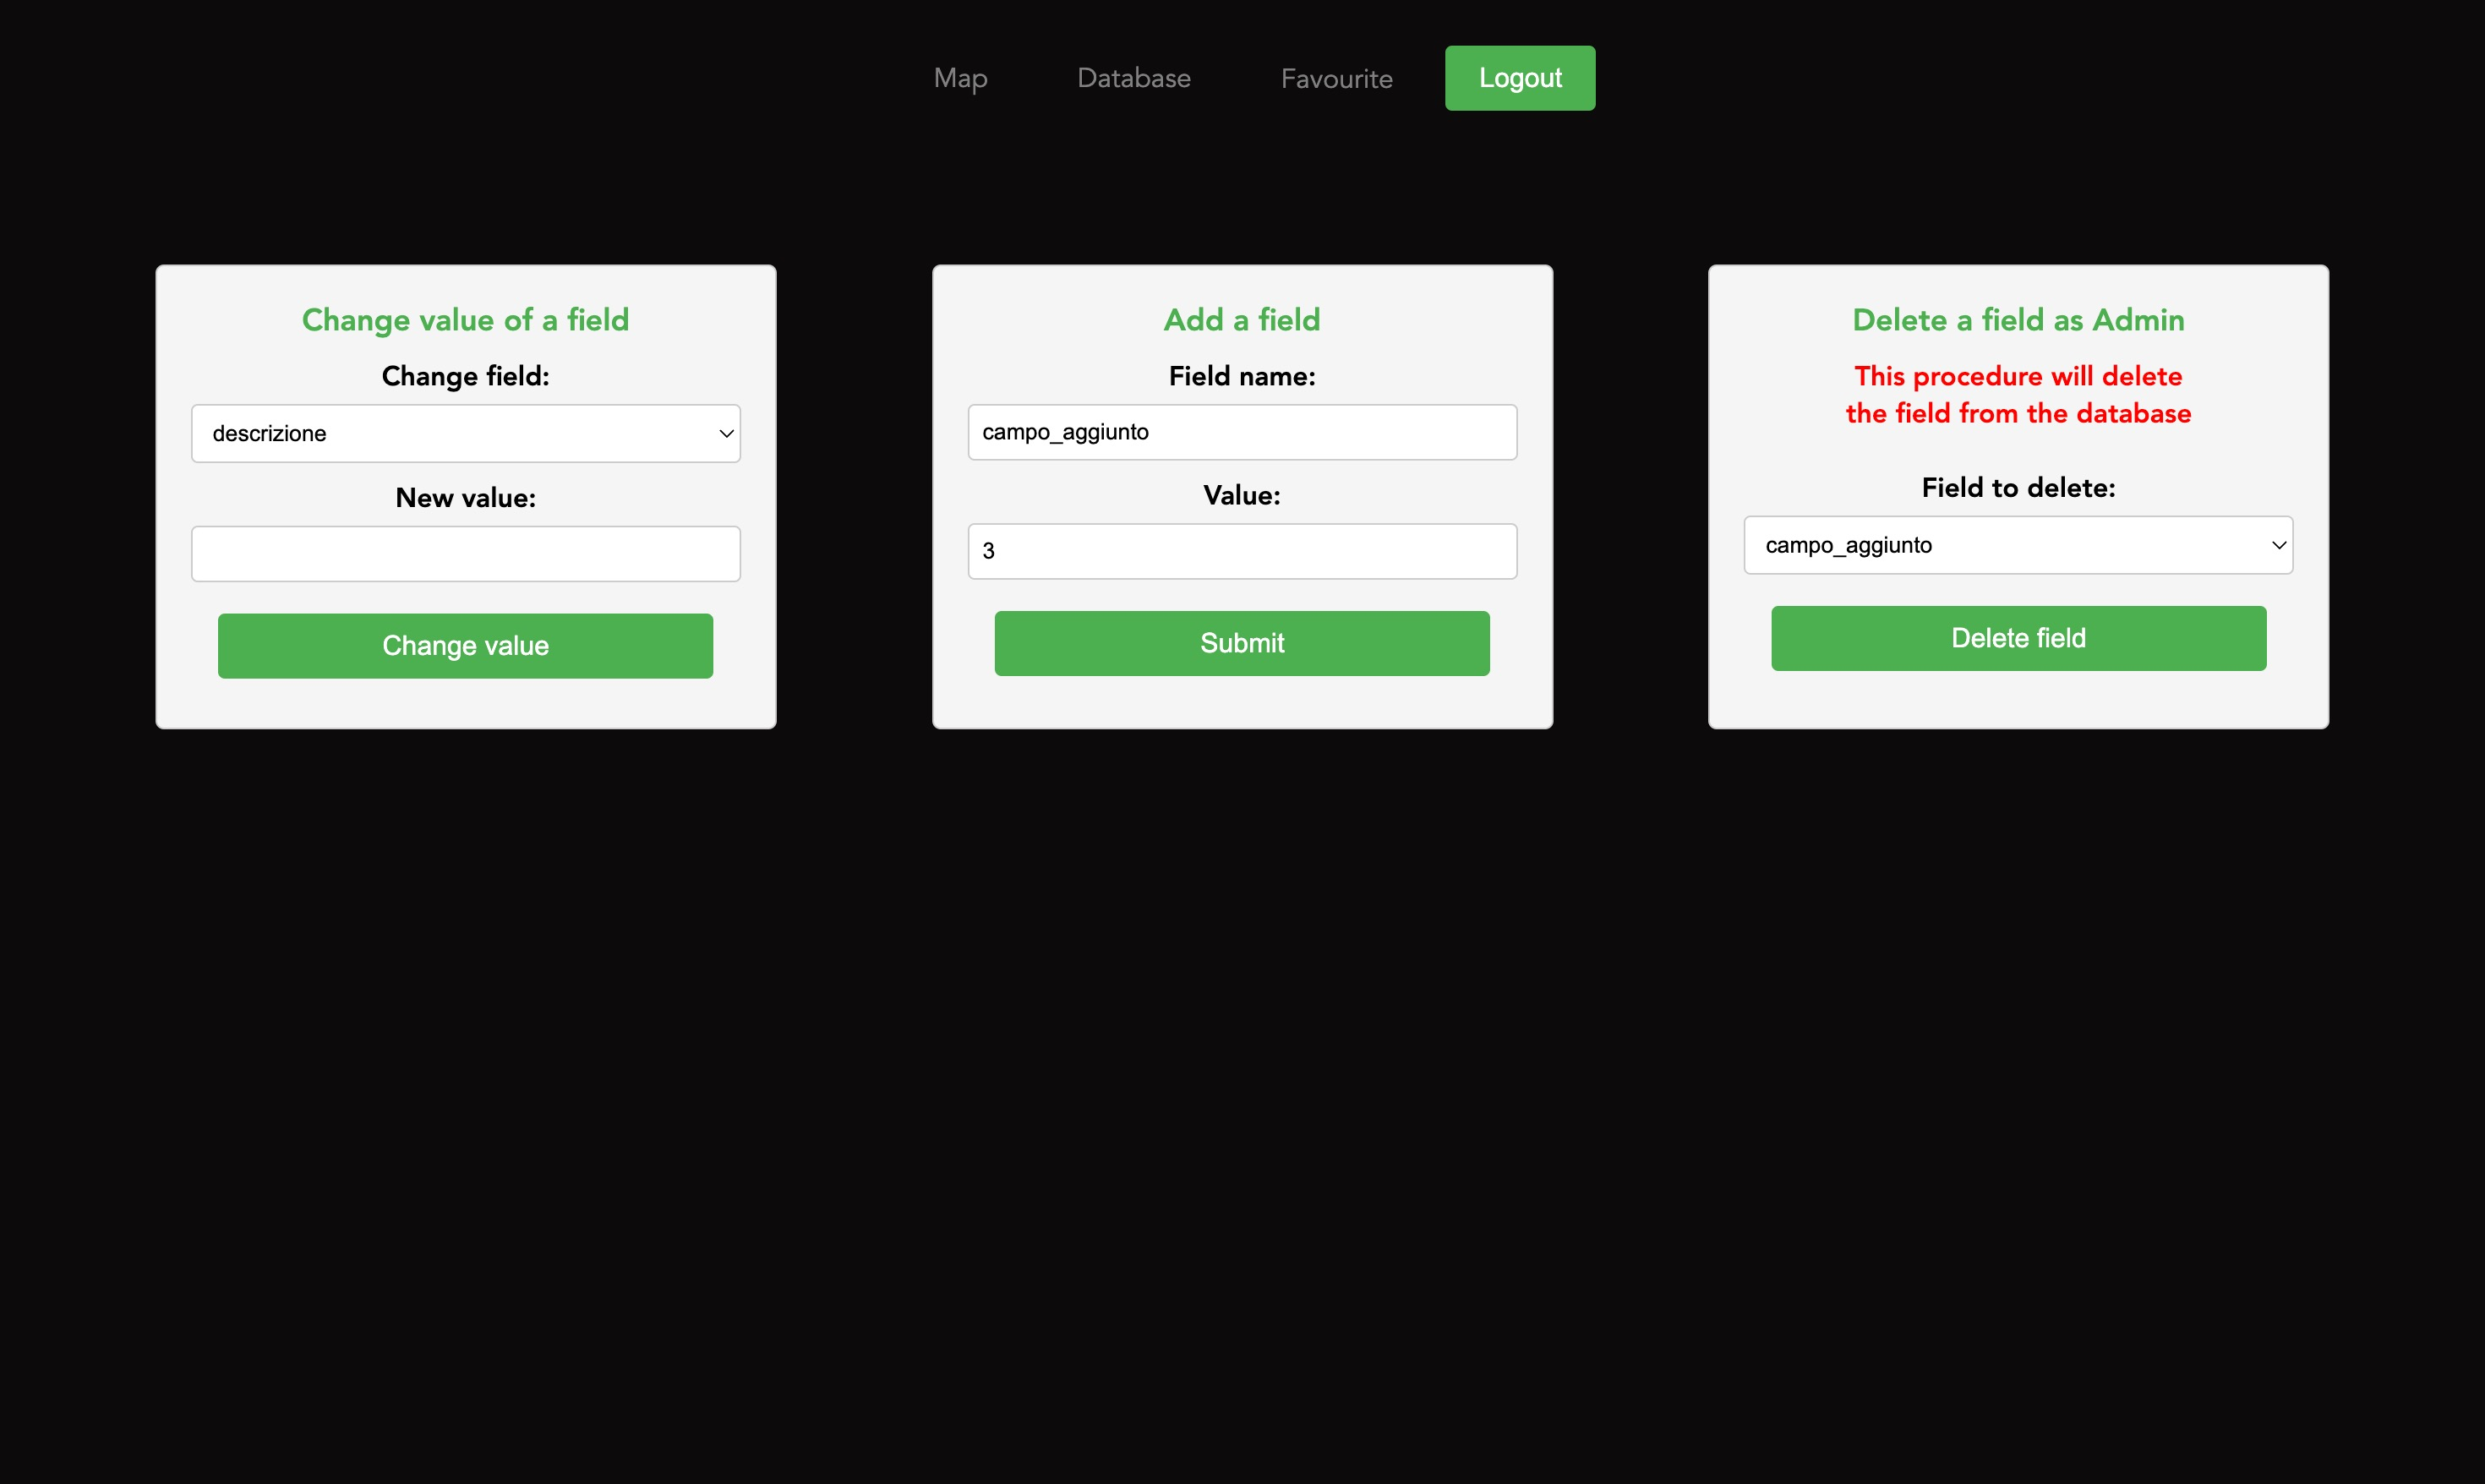
\includegraphics[width=13cm]{images/Extra_field.jpg}
\caption[Pagina per aggiungere informazioni sui punti di interesse]{Pagina per aggiungere informazioni sui punti di interesse}\label{fig:extra_field}
\end{center}
\end{figure}

Questa pagina presenta tre opzioni:

\begin{itemize}
    \item Cambiare valore ad un campo

    Selezionando un campo dal menù a tendina è possibile cambiarne il valore. Questa funzione è utilizzabile per tutti gli utenti.

    \item Aggiungere un campo

    È possibile aggiungere un campo a quel punto di interesse mettendogli il nome nella prima casella e il valore nella seconda. Nel caso verrà inserito un campo già presente nel punto, il valore di questo verrà sovrascritto. Questa funzione è utilizzabile per tutti gli utenti.

    \item Eliminare un campo

    È possibile eliminare un campo aggiunto dagli utenti dal punto di interesse. Questa funzione è utilizzabile solo per gli amministratori.
\end{itemize}
